\documentclass[a4paper, english, 11pt, twoside]{memoir}

\usepackage[T1]{fontenc}
\usepackage[utf8]{inputenc}
\usepackage[english]{babel}

\usepackage{amsmath, amssymb}

\usepackage{color}

\usepackage{float}

\usepackage{graphicx}

\usepackage{parskip}

\usepackage[colorlinks=true, urlcolor=blue, citecolor=blue, linkcolor=black]{hyperref}

% Bibliography

\usepackage[backend=bibtex, backref=true, style=numeric, sorting=none, minnames=4, maxnames=4, minbibnames=4, maxbibnames=4, mincitenames=4, maxcitenames=4]{biblatex}
\addbibresource{bibliography.bib}

% Table of contents

% \setsecnumdepth{subsubsection}
% \maxtocdepth{subsubsection}
\setsecnumdepth{subsection}
\maxtocdepth{subsection}

% Fonts

\usepackage{lmodern}
\usepackage{calligra}
\renewcommand{\familydefault}{\sfdefault}

% Background image

\usepackage{eso-pic}

% Caption

\usepackage{caption}
\captionsetup{font=footnotesize, labelfont=footnotesize}

% Geometry

\usepackage[top=1.3in, bottom=1.3in, left=1.in, right=1.in]{geometry}

% Line height

\linespread{1.1}

% Header

\let\footruleskip\undefined
\usepackage{fancyhdr}
\pagestyle{fancy}
\fancyhead[LO, RE]{\nouppercase{\leftmark}}
\fancyhead[RO, LE]{\thepage}
\fancyfoot{}

% Arrays

\renewcommand{\arraystretch}{1.5}

% Sign operator

\DeclareMathOperator{\sign}{sgn}

% Commands

\newcommand{\todo}[1]{\begin{center} \color{red} \textbf{TODO:} #1 \end{center}}

\newcommand{\GeVc}{GeV c$ ^{-1} $}
\newcommand{\um}{$ \mu $m}
\newcommand{\us}{$ \mu $s}
\newcommand{\pT}{$ p_T $}
\newcommand{\pZ}{$ p_Z $}
\newcommand{\axis}[1]{#1}

%

\title{Development of a Triple-GEM detector system for the upgrade of the forward region of the muon spectrometer of the CMS experiment at LHC}
\author{Thomas LENZI}
\date{}

\begin{document}

\frontmatter

{ \pagestyle{empty}

	\maketitle

	\cleardoublepage

	% \vspace*{2cm}

\begin{flushright}
	{ \Large \calligra }
\end{flushright}

	% \cleardoublepage

}

\setcounter{page}{1}

{ \pagestyle{plain}

	\addcontentsline{toc}{chapter}{Abstract}

\begin{abstract}

	In the upcoming years, with the upgrade of the LHC to higher luminosities, CMS will be subject to an increasing flux of particles, especially in its most forward region, at $ | \eta | $ > 1.6. To consolidate the muon spectrometer of CMS and increase redundancy, the CMS GEM collaboration proposes to instrument the 1.6 < $ | \eta | $ < 2.1 region, originally foreseen to be equipped with RPC, with Triple-GEM detectors. This technology has proven to remain efficient under high fluxes and meets the requirements of CMS. \\

	This work, using simulations, studies three track reconstruction algorithms intended to be installed in the first selection stage of CMS for Triple-GEM detectors: a Least Squares fit, a standard Kalman filter, and a modified Kalman filter. A comparative analysis is performed between the results obtained with Triple-GEM detectors and those yielded by the actual system in order to quantify the improvements made to the CMS muon spectrometer and to the CMS trigger system. \\

\end{abstract}

\renewcommand{\abstractname}{Résumé}

\begin{abstract}

	Dans les années à venir, avec la mise à niveau du LHC pour de plus hautes luminosités, CMS sera soumis à un flux croissant de particules, surtout dans la région avant, à $ | \eta | $ > 1.6. Afin de consolider le spectromètre à muons de CMS et d'augmenter la redondance, la collaboration CMS GEM propose d'installer des détecteurs Triple-GEM dans la région 1.6 < $ | \eta | $ < 2.1, qui devait initialement être équipée de RPC. Les Triples-GEMs peuvent resister à des flux intenses sans perdre de leur efficacité et ainsi satisfaire aux exigences de CMS. \\

	Ce travaille étudie, à l'aide de simulations, trois algorithmes de reconstruction de traces destinés à être installés dans le premier niveau de déclenchement de CMS: un Moindres Carrés, un filtre de Kalman standard et un filtre de Kalman modifié. Une analyse comparative est faite entre les résultats obtenus en utilisant les Triple-GEMs à ceux résultant du système actuel afin de caractériser l'impact des différents algorithmes sur le spectromètre à muons et sur le système de déclenchement de CMS.

\end{abstract}

\vfill
\textbf{Keywords:} GEM, Leve1 Trigger, CMS, Upgrade, muon detectors

	\cleardoublepage

	\tableofcontents
	\cleardoublepage

	% \chapter*{Acknowledgment}
\addcontentsline{toc}{chapter}{Acknowledgment}
\label{chap:acknowledgment}

	% \cleardoublepage

}

\mainmatter

	\chapter*[Introduction]{Introduction}
\addcontentsline{toc}{chapter}{Introduction}
\label{chap:introduction}

	\cleardoublepage

	\chapter{The Large Hadron Collider and the CMS Experiment}
\label{chap:lhc_cms}

    The first section of this chapter is dedicated to the \emph{Large Hadron Collider} (LHC), a hadron accelerator and collider. We will present the injection chain which provides the LHC with a particle beam, the relevant parameters needed to describe the collisions, and the run schedule and upgrades foreseen for the upcoming years. \\

    The second section of this chapter is devoted to the \emph{Compact Muon Solenoid} (CMS) experiment, one of the four main experiments exploiting the LHC beam. We start by giving an overview of the detector and its geometry, and then proceed by describing the sub-detectors that comprise CMS as well as its trigger and \emph{Data Acquisition} (DAQ) system.

    \section{The Large Hadron Collider}

        The LHC \Cite{Evans:1129806} is state-of-the-art in particle accelerators and colliders engineering. Built at and by the \emph{European Organization for Nuclear Research} (CERN), it is located in the 26.7 km long tunnel that previously hosted the \emph{Large Electron Positron} collider (LEP). Using smaller accelerators as injectors, it is designed to accelerate and collide protons or heavy ions at energies up to 14 TeV in the center of mass reference frame. These collisions take place at four different locations where the ALICE \Cite{1748-0221-3-08-S08002}, ATLAS \Cite{1748-0221-3-08-S08003}, CMS \Cite{1748-0221-3-08-S08004}, and LHCb \Cite{1748-0221-3-08-S08005} experiments collect and analyse data.

        \subsection{Timeline}

            In 2003, the first section of the accelerator was assembled inside the tunnel. The construction continued until 2008 when the last piece was mounted and the LHC was complete and ready to produce its first collisions. After a successful preliminary run in August an incident occurred shutting down the machine for nearly one year. \\

            Since then, the LHC is slowly building up in energy, reaching 8 TeV in the center of mass reference frame before the \emph{Long Shutdown-1} (LS1) which started at the beginning of 2013. This 20 months long period will be used to perform maintenance and to upgrade the LHC as well as the experiments, and to prepare them to run at nominal energy and luminosity.

        \subsection{Injection Complex}

            Before being accelerated and collided by the LHC, the protons and ions are produced and sped up by multiple accelerators. Figure \ref{fig:lhc_cms__lhc_injection_chain} depicts the injection chain of the LHC. The first element in this chain is the \emph{Linac2}, which produces protons by ionizing gaseous hydrogen. These protons are accelerated and regrouped into bunches by a set of magnets before being transferred to the \emph{Proton Synchrotron Booster} (Booster), \emph{Proton Synchrotron} (PS), and \emph{Super Proton Synchrotron} (SPS), which furthermore increase the bunches' energy. Finally, the particles enter the LHC through two different tubes travelling in opposite directions.

            \begin{figure}[h!]
                \centering
                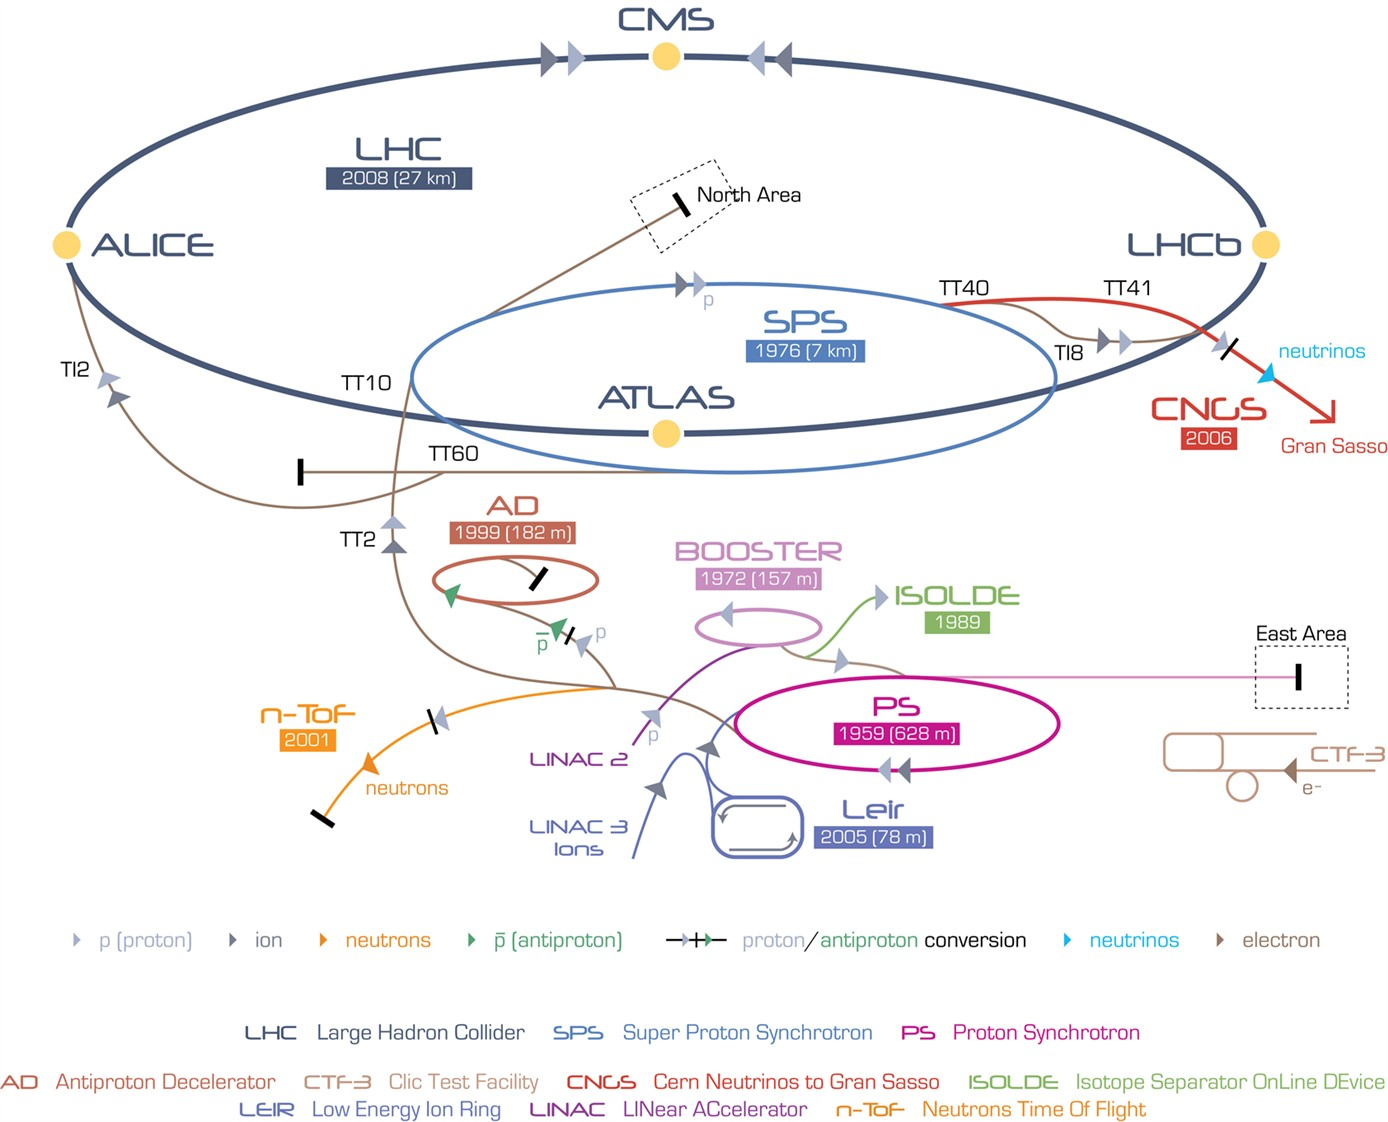
\includegraphics[width = 12cm]{lhc_cms/lhc_injectors.jpg}
                \caption{Schematic representation of the LHC's injection chain composed of multiple smaller accelerators \Cite{TE-EPC-LPC_in_LHC}.}
                \label{fig:lhc_cms__lhc_injection_chain}
            \end{figure}

        \subsection{Beam Structure and Luminosity}

            As previously mentioned, the particle beam is not a continuous flux of protons but rather a series of bunches that travel along the tube and are accelerated, regrouped, and focused by a set of magnets. Once they achieve the desired energy they are collided at a frequency of 40 MHz at the four crossing sites. \\

            The LHC also delivers a high instantaneous luminosity $ \mathcal{L} $ which is essential to detect rare processes as it yields the apparition's frequency of events in a given interaction process
            \begin{equation}
                f_{process} = \mathcal{L} \sigma_{process} \ ,
            \end{equation}
            where $ f_{process} $ is the number of expected events per second, and $ \sigma_{process} $ is the interaction cross-section of the process. For a circular collider, the instantaneous luminosity is defined as
            \begin{equation}
                \mathcal{L} = \frac{\gamma N^2_b n_b f_{rev}}{4 \pi \epsilon_n \beta^*} F \ ,
                \label{eq:lhc_cms__luminosity}
            \end{equation}
            where $ N_b $ is the number of protons or ions per bunch, $ n_b $ is the number of bunches per beam, $ f_{rev} $ is the revolution frequency, $ \gamma $ is the Lorentz factor, $ \epsilon_n $ is the beam emittance, $ \beta^* $ is the beta function at the \emph{Interaction Point} (IP), and $ F $ is a function of the crossing angle between the beams at the IP. The $ \epsilon_n $ and $ F $ parameters are related to the bunches' structure and more specifically to their spatial spreading. These parameters change during the machine's operation as the number of protons per bunch decreases, and the bunches spread out. We can integrate $ \mathcal{L} $ over a long period of time in order to get the integrated luminosity
            \begin{equation}
                L = \int \mathcal{L} \ dt \ ,
            \end{equation}
            which results in the number of events we can expect for a given interaction process
            \begin{equation}
                N_{process} = L \sigma_{process} \ .
                \label{eq:lhc_cms__N}
            \end{equation}

        \subsection{Future Plans and Upgrades}

            The LHC's operation plan is divided in two phases: phase 1 during which the machine will slowly reach its nominal capabilities, and phase 2 where the machine will run at even higher luminosity after undergoing a major upgrade. \\

            Phase 1 extends from 2010 to about 2020 and is divided into three shorter periods separated by two Long Shutdowns. Table \ref{tab:lhc_cms__lhc_performances} shows the energy and luminosity at which the LHC will be running after both maintenances (LS1 and LS2). While the machine is shut down, physicists will have access to the detectors and will be able to perform repairs and upgrades. \\

            \begin{table}[h!]
                \centering
                \begin{tabular}{l|c|c}
                    Period & Energy & Luminosity \\ \hline
                    2010-2012 & 7-8 TeV & 0.5 10$ ^{34} $ cm$ ^{-2} $ s$ ^{-1} $ \\
                    Long Shutdown 1 (LS1) & - & - \\
                    2015-2017 & 13-14 TeV & 10$ ^{34} $ cm$ ^{-2} $ s$ ^{-1} $ \\
                    Long Shutdown 2 (LS2) & - & - \\
                    2019-2021 & 14 TeV & 2 10$ ^{34} $ cm$ ^{-2} $ s$ ^{-1} $
                \end{tabular}
                \caption{Energy and luminosity of the LHC during the different periods of phase 1 \Cite{Evans:1129806}.}
                \label{tab:lhc_cms__lhc_performances}
            \end{table}

            After LS1, the energy will be increased by using the magnets at full capability, and the luminosity will be multiplied by a factor of two by bringing down the time between two collisions to 25 ns instead of 50 ns. The luminosity will further be increased after LS2 when the machine enters the \emph{High Luminosity LHC} (HL-LHC) era. As reviewed in Equation \ref{eq:lhc_cms__luminosity}, various parameters can be tuned in order to achieve that goal. The main possibilities are to \Cite{Koutchouk:1306815}
            \begin{enumerate}
                \item increase the number of bunches $ \sim n_b $;
                \item increase the number of protons per bunch by making them longer $ \sim N_b $;
                \item increase the collisions' frequency $ \sim f_{rev} $;
                \item decrease the bunches' spread by improving the efficiency of the focusing magnets $ \sim \epsilon_n $;
                \item decrease the collisions' angle by adding magnets near the IPs $ \sim F $. \\
            \end{enumerate}

            Phase 2 involves a major upgrade of the LHC and of the injection chain which would occur during LS3 after 2021. The objective is to increase the luminosity by a factor of 10 to reach 10$ ^{35} $ cm$ ^{-2} $ s$ ^{-1} $.

    \section{The CMS Experiment}

        CMS \Cite{1748-0221-3-08-S08004} is, along with ATLAS, ALICE, and LHCb, one of the four main experiments recording the LHC beam collisions. Its structure and components are depicted in Figure \ref{fig:lhc_and_cms__cms_global_view}. As represented, it is composed of five main parts: the \emph{silicon tracker} (TK) in blue, the \emph{electromagnetic calorimeter} (ECAL) in green-blue, the \emph{hadronic calorimeter} (HCAL) in orange, the \emph{magnet} in purple, and the \emph{muon chambers} in white. \\
        
        \begin{figure}[h!]
            \centering
            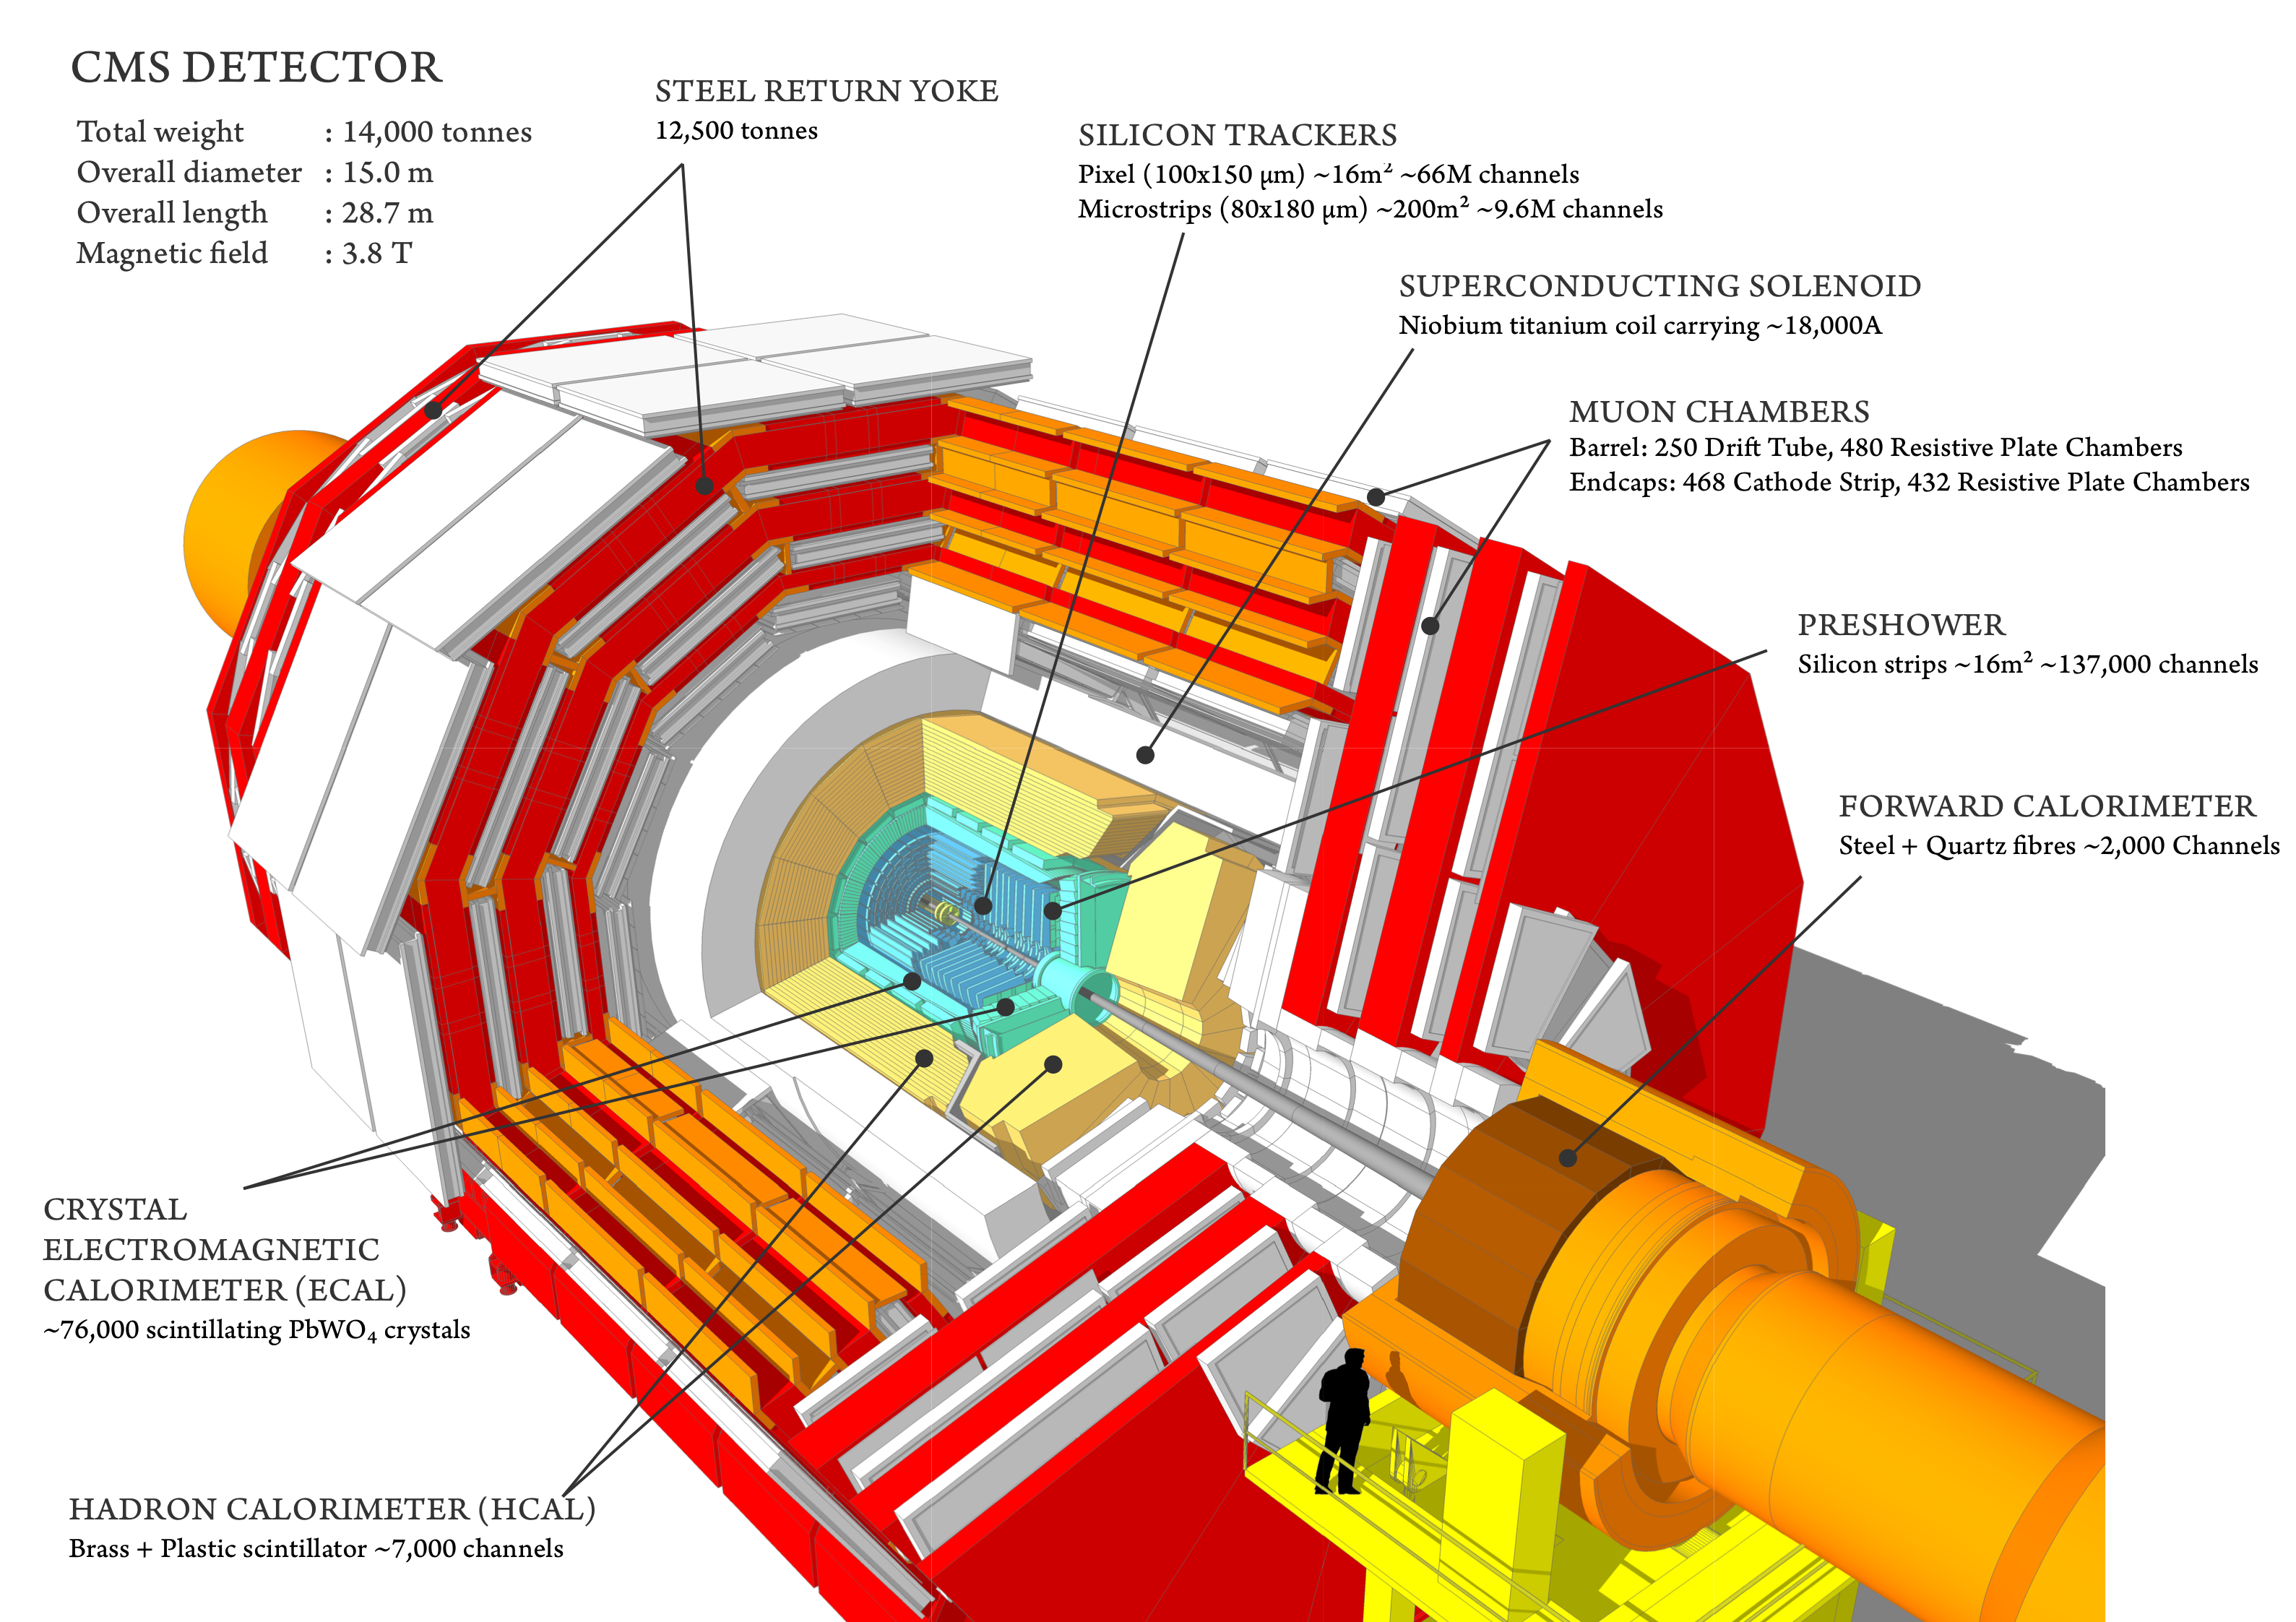
\includegraphics[width = 16.5cm]{lhc_cms/cms_global_view.png}
            \caption{Representation of CMS and its different parts: the silicon tracker (blue), the electromagnetic calorimeter (green-blue), the hadronic calorimeter (orange), the magnet (purple), and the muon chambers (white) \Cite{Fig:cms-detector-design}.}
            \label{fig:lhc_and_cms__cms_global_view}
        \end{figure}

        CMS is divided into two regions: the barrel where the detectors are laid out cylindrically around the beam, and the endcaps where the detectors are placed perpendicularly to the beam. Although CMS has the ability to detect a wide range of interaction channels, it is characterized by its effective trigger system for muons and its strong magnetic field, which gave its name to the detector.

        \subsection{Detector Geometry}

            As CMS is of the cylindrical type, appropriate coordinates are defined to track particles. The Cartesian coordinates \axis{X}, \axis{Y}, and \axis{Z} are first set: \axis{X} points to the center of the accelerator, \axis{Y} to the surface, and \axis{Z} in the direction of the beam, as illustrated in Figure \ref{fig:lhc_and_cms__cms_coordinates}. The \axis{XY} plane is also referred to as the transverse plane. The problem with this set of coordinates is that the physics is not symmetrical under these, which would be a beneficial feature. Therefore, the rapidity $ y $, a Lorentz invariant over which the particles in the final state are equally distributed, is used. The rapidity is defined as 
            \begin{equation}
                y = \frac{1}{2} \ln \left( \frac{E + p_Z}{E - p_Z} \right) \ ,
            \end{equation}
            which for highly relativistic particles can be approximated by the pseudo-rapidity
            \begin{equation}
                \eta = - \ln \left[ \tan \left( \frac{\theta}{2} \right) \right] \ ,
            \end{equation}
            where $ \theta $ is the polar angle (angle between the particle and the \axis{Z} axis). The other coordinates are the azimuth $ \phi $ (angle in the \axis{XY} plane), and the distance to the beam in the transverse plane $ R $ for tracks the barrel, and the \axis{Z} coordinate for tracks the endcaps. \\

            \begin{figure}[h!]
                \centering
                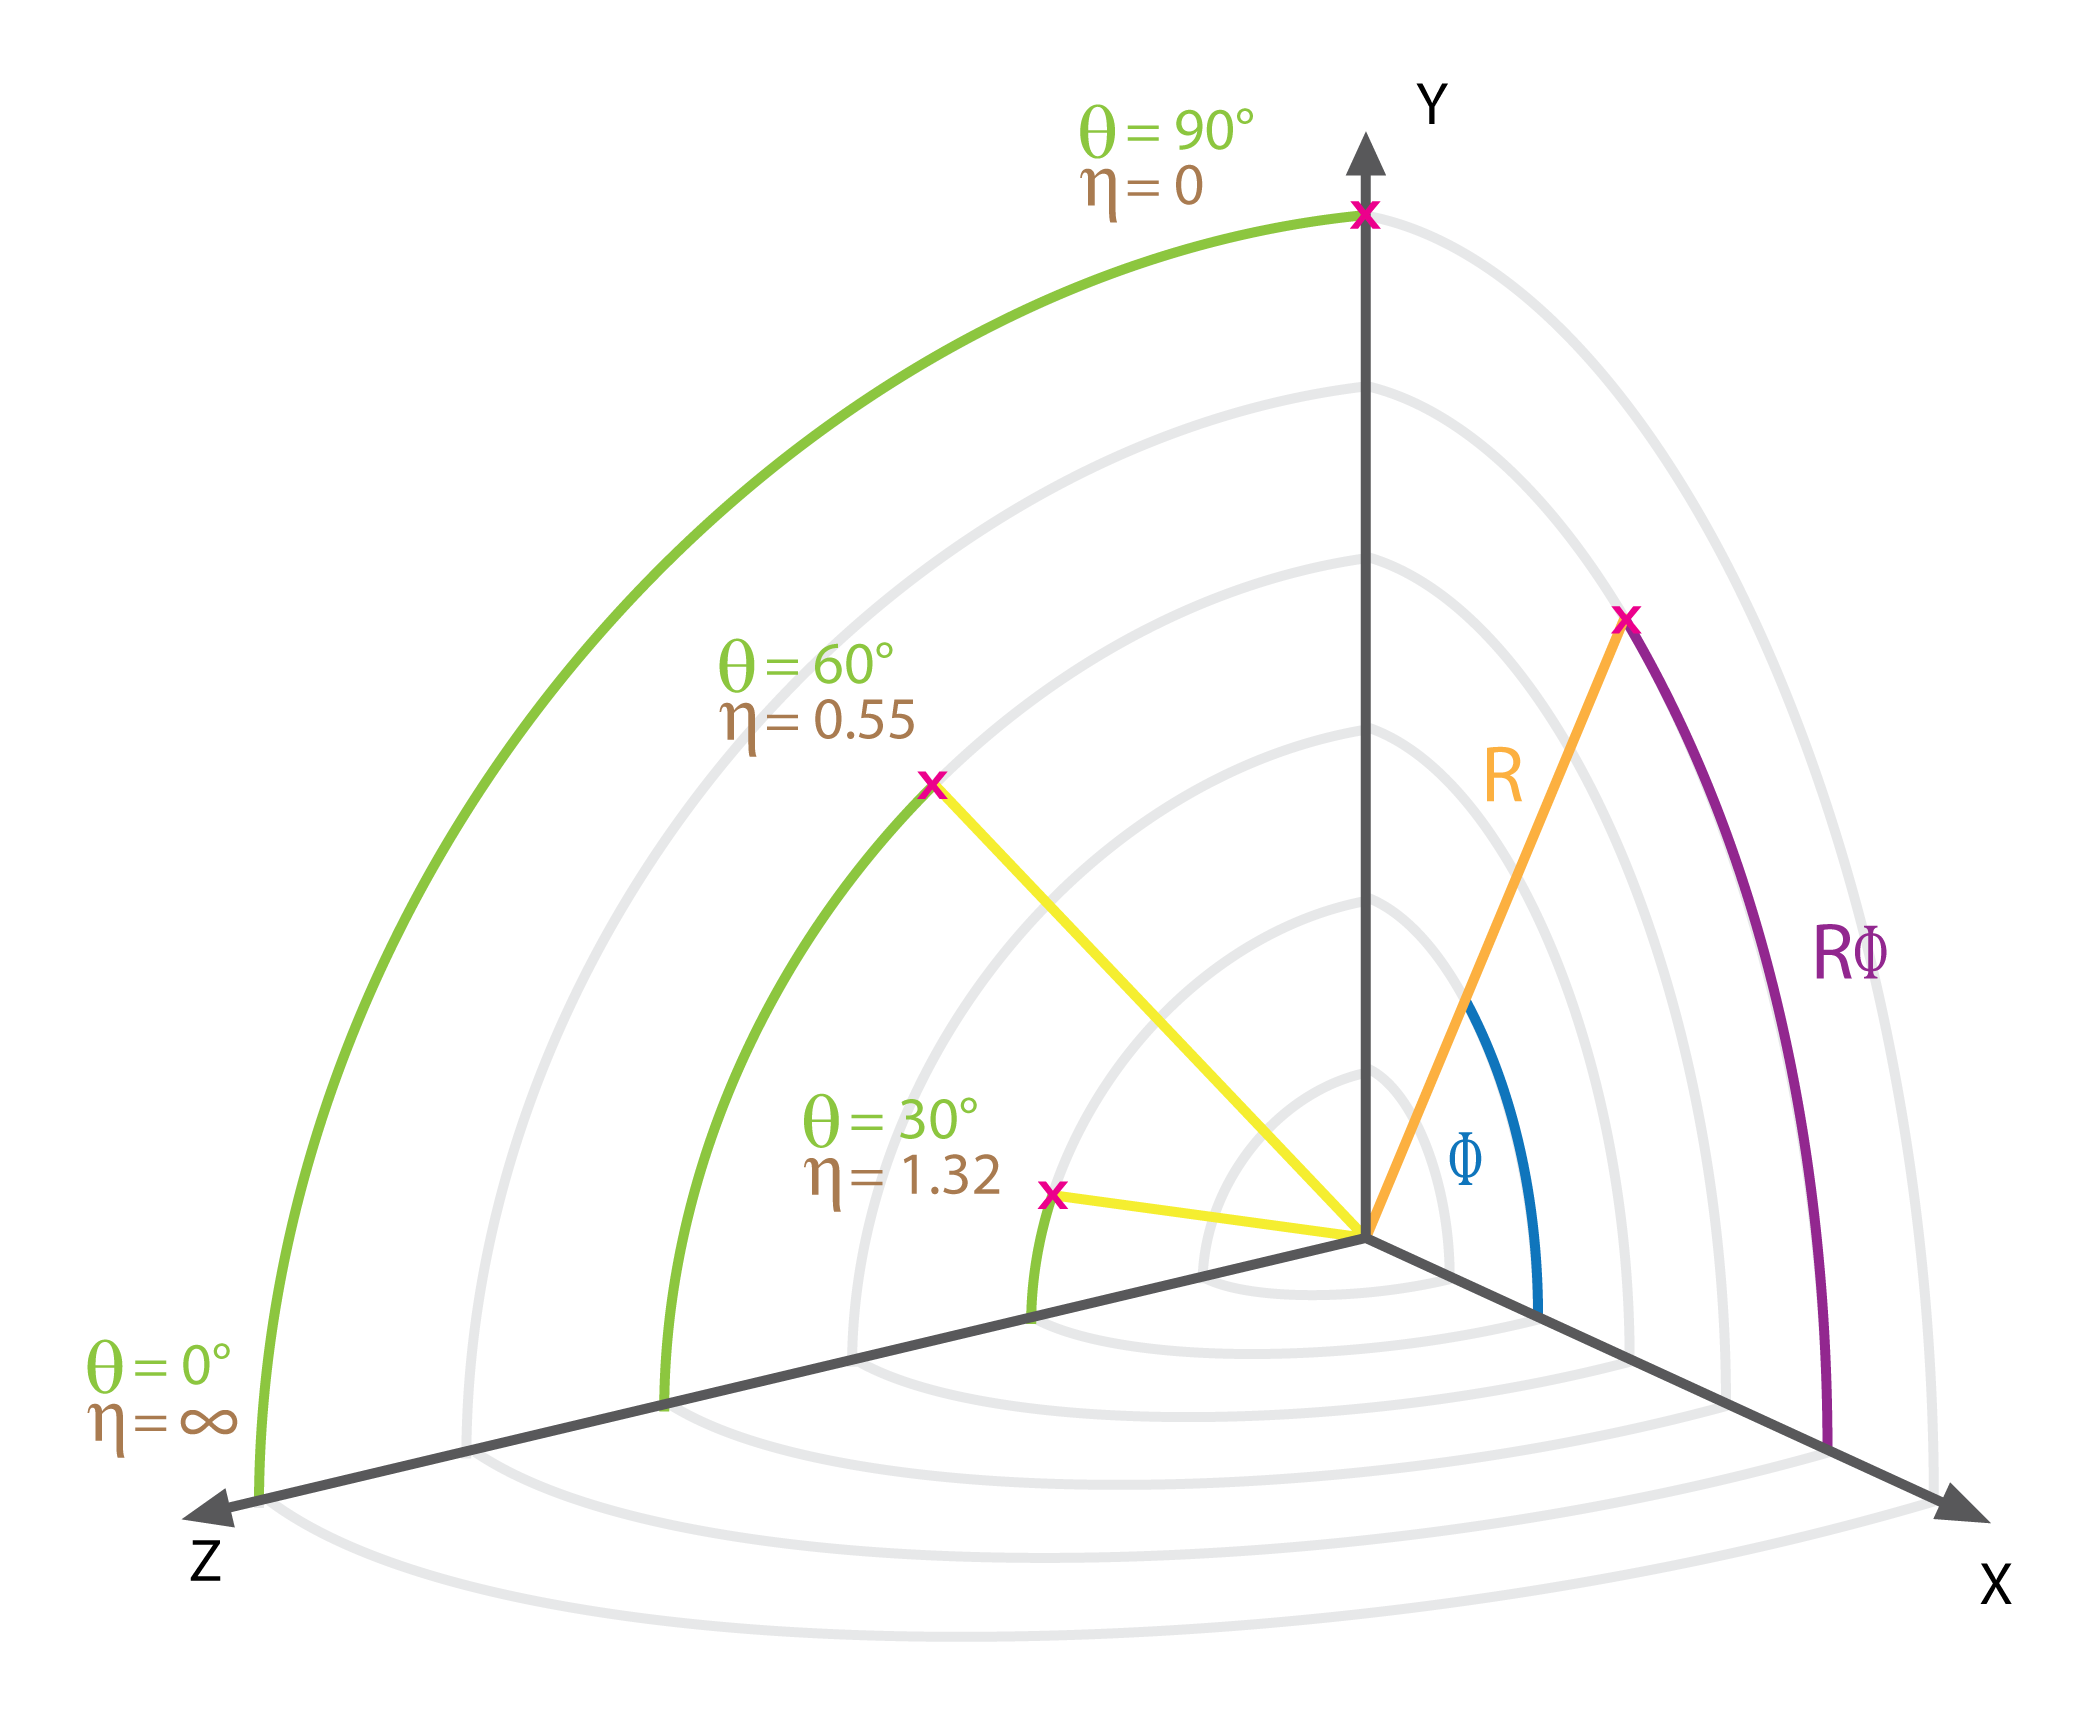
\includegraphics[width = 11cm]{lhc_cms/cms_coordinates.png}
                \caption{Pseudo-rapidity $ \eta $ and azimuthal angle $ \phi $ used to track particles inside CMS.}
                \label{fig:lhc_and_cms__cms_coordinates}
            \end{figure}        

            As previously stated, the particles in the final state are equally distributed over $ \eta $. This means that the particles fluxes are lower in the barrel than in the endcaps. This impacts the detectors' geometry.

        \subsection{Tracking System}

            The silicon tracker is the detector closest to the IP. It is composed of two different types of semiconductor detectors: \emph{silicon pixels} and \emph{silicon strips}. These detectors have an excellent spatial resolution (down to 25 \um{}) which yields excellent momentum reconstruction capabilities (resolution of the order of 1\% at low transverse momenta). The disposition of the different technologies is represented in Figure \ref{fig:lhc_and_cms__cms_tracker}. The silicon pixels are represented in blue, while TIB, TID, TOB, and TEC refer to different regions of the silicon strip detector. \\

            \begin{figure}[h!]
                \centering
                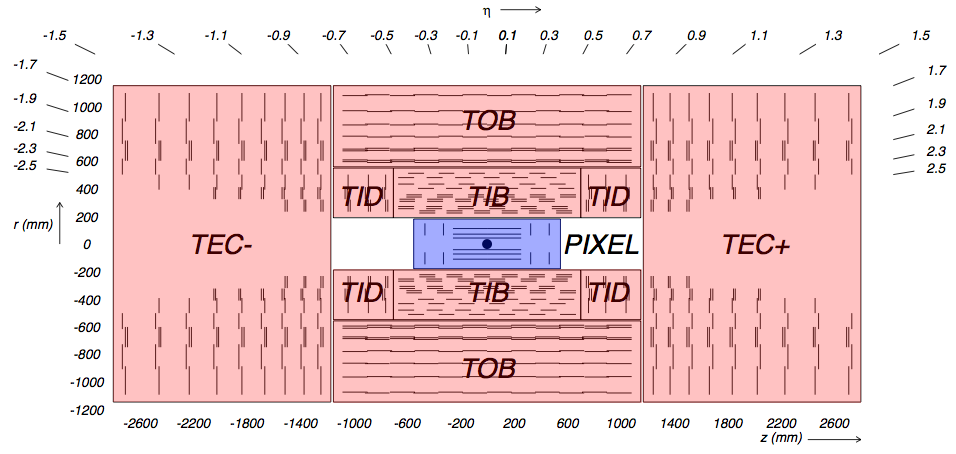
\includegraphics[width = 13cm]{lhc_cms/cms_tracker_view.png}
                \caption{Disposition of the different detectors in the silicon tracker. PIXEL (blue) refers to silicon pixel detectors while TIB, TID, TOB and TEC (red) all refer to silicon strip detectors \Cite{CMS_at_LHC}.}
                \label{fig:lhc_and_cms__cms_tracker}
            \end{figure}

            Semiconductor detectors are made out of two pieces of silicon, one negatively doped containing more unbounded electrons, and one positively doped containing more unbounded holes (absence of electrons), put together to form a n-p junction. At the interface, the electrons and the holes diffuse in the opposite region and recombine with the particles of opposite charge, creating an unbalance in charge: the n region and p region close to the junction become, respectively, positively and negatively charged. From this, an electric field is formed which slows the diffusion down until the system reaches equilibrium. When a charged particle passes through this region and losses energy, electrons switch from non-conductive to conductive bands creating electrons/holes pairs. Under the action of the electric field, they migrate towards the n or p regions and form the signal on the readout electronics. Unfortunately, the number of unbounded charges is still high compared to the formed signal and the active region is small. To increase the detection efficiency, a voltage difference is applied to the semiconductor further diffusing the electrons and holes through the junction. Typically, for a voltage difference of 100 V, the size of the active region is of the order of 300 \um{}.

            \subsubsection{Pixel Detectors}

                The silicon pixels detectors, represented in Figure \ref{fig:lhc_and_cms__cms_pixel_detector}, are composed of small 100 \um{} x 150 \um{} rectangles of readout material disposed on a block of detection medium formed by a n-p region. The electrons are formed in that region and migrate towards the silicon pixels. The challenge arising is that each pixel needs its own readout electronics which takes a significant amount of space and requires output cables. These cables prevent the placing of detectors which creates dead-zones. Physicists and engineers must find the right balance between the number of pixels (granularity), the size of the electronic, and the detectors' resolution. \\

                \begin{figure}[h!]
                    \centering
                    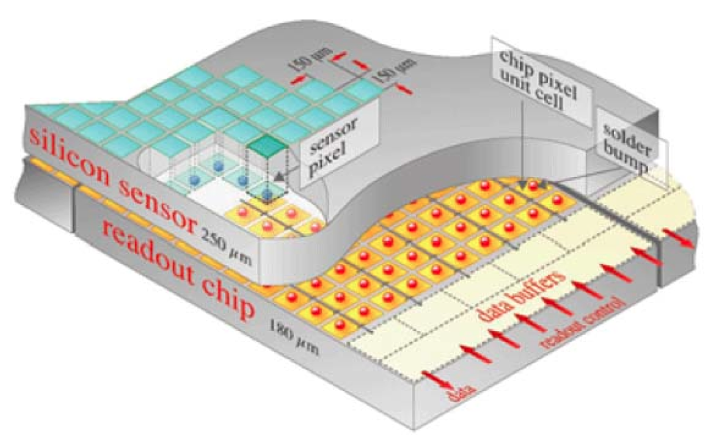
\includegraphics[width = 8cm]{lhc_cms/cms_tracker_pixel.png}
                    \caption{Disposition of the readout pixels (orange and red) on the same detection block (gray) inside a silicon pixel detector \Cite{CMS_Tracker_Construction}.}
                    \label{fig:lhc_and_cms__cms_pixel_detector}
                \end{figure}    

                Nevertheless, the pixel detectors are the most precise tracking technology in CMS with a spatial resolution of 15 to 20 \um{}. This value is smaller than the size of the pixels because of \emph{charge sharing}. All the pixels sharing the same detection block also share the energy deposited by a particle. By reading the total deposited charge on each of the pixels, we can find the \emph{Center of Gravity} (COG). The COG method is based on the assumption that there exists a linear relation between the induced pulse's height on a pixel and the distance between its center and the particle's hit, so that each pixel is assigned a weight proportional to the deposited charge. The reconstructed coordinate $ \mathbf{x}_{COG} $ of the cluster is then given by 
                \begin{equation}
                    \mathbf{x}_{COG} = \frac{\sum_i \mathbf{x}_i q_i}{\sum_i q_i} \ ,
                    \label{eq:lhc_and_cms__charge_sharing}
                \end{equation}
                where $ q_i $ is the individual pixel signal in the cluster, and $ \mathbf{x}_i $ is the positions of the pixel in the defined coordinate system. The same technique can be applied to other detectors as long as the charge is read out analogically and not digitally\footnote{One can consider using the same method with digital readouts but will not be able to achieve the same resolutions.}.           
            

            \subsubsection{Strip Detectors}

                The most outer layers of the tracker cannot have a granularity as high as the pixel detectors, for both financial and technical reasons. The amount of data that would have to be read out is considerable, and the technology to do so is not yet available. A way to reduce the granularity of the detectors is to measure only one coordinate by using silicon strips instead of pixels. The strips are separated by 80 to 122 \um{} which gives a resolution between 23 \um{} and 53 \um{} in the direction perpendicular to the strips. Unfortunately, as expected, there is a larger error on the other coordinate (along the strip) corresponding to the size of the detection cell. To improve global precision, some of the cells have two strip detectors placed with a small stereo angle, typically 100 mrad, allowing them to measure both coordinates. However, this set up generates \emph{ghosts} because of the ambiguity created when more than one particle hits the detector at the same time.
            
            \subsubsection{System Performances}  
            \label{sec:lhc_and_cms__tracker_system_performances}        

                Due to the magnetic field generated by the solenoid, the trajectories charged particles are bent inside the tracker. The relation between the bending radius of the track $ R $ , the transverse momentum $ p_T $, and the intensity of the magnetic field $ B $ is
                \begin{equation}
                    R[\mbox{m}] = \frac{p_T[\mbox{GeV c}^{-1}]}{0.3 B[\mbox{T}]} \ .
                    \label{eq:lhc_and_cms__radius_to_momentum_relation}
                \end{equation}
                By measuring the bending radius of the track and inverting the previous relation, the transverse momentum of the particles can be obtained. Tracks created by high energy particles will be straighter than those left by low energy particles and therefore more difficult to reconstruct. \\

                As previously stated, the tracker offers an excellent resolution on the position of the particles and therefore gives precise measurements of the particles' momentum. Figure \ref{fig:lhc_and_cms__cms_tracker_performances} shows the resolution on the transverse momentum \pT{} (left) and detection efficiency (right) of the tracker as a function of the pseudo-rapidity $ \eta $ for muons of transverse momenta \pT{} of 1, 10, and 100 \GeVc{}. The resolution is less than 1\% for muons of 1 and 10 \GeVc{} in the barrel ($ \eta $ < 1) and quickly rises in the most forward region. The same effect is observed for the detection efficiency which is close to 100\% in the barrel but significantly diminishes at higher pseudo-rapidities. Precision decreases in the most forward region where the strip pitch is greater and more material is present, causing more scatterings.

                \begin{figure}[h!]
                    \centering
                    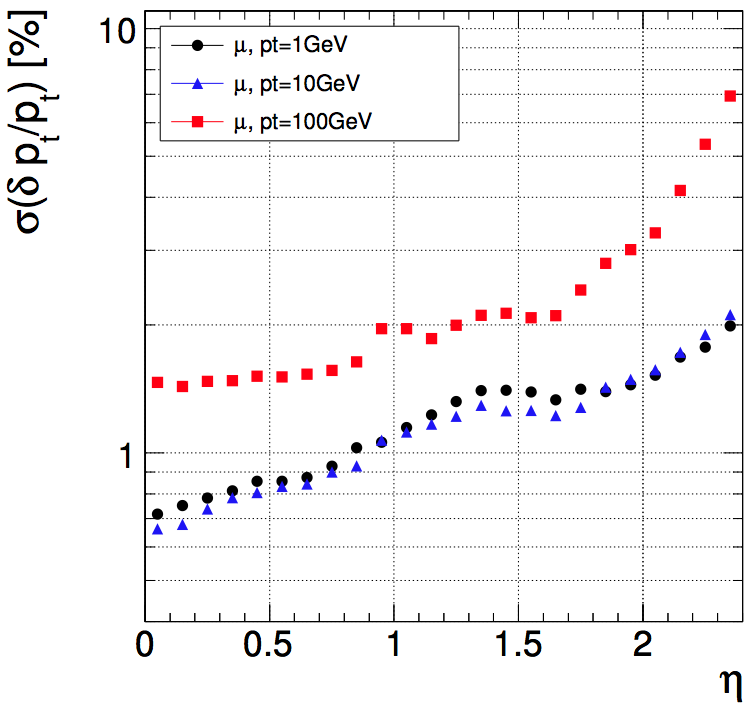
\includegraphics[width = 6.3cm]{lhc_cms/cms_tracker_resolution.png}
                    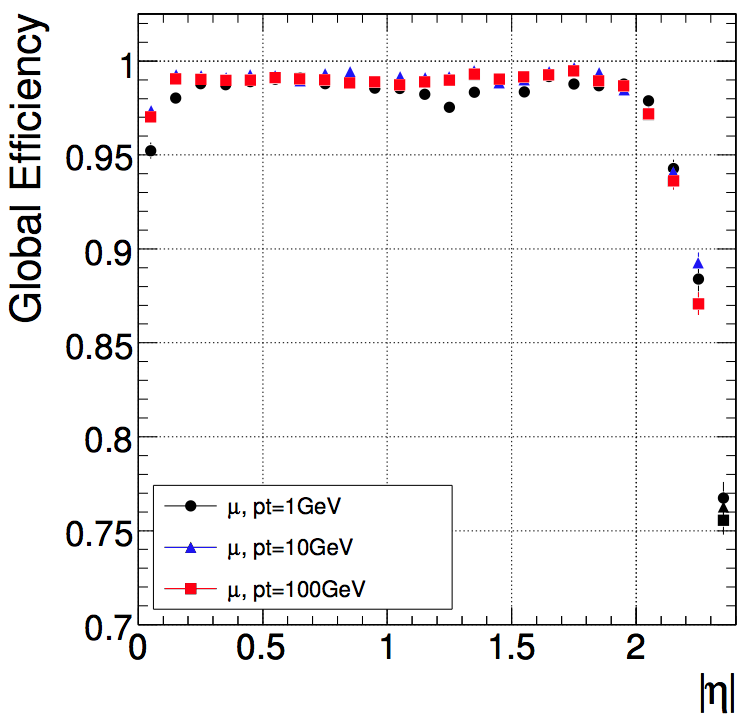
\includegraphics[width = 6.3cm]{lhc_cms/cms_tracker_efficiency.png}
                    \caption{Resolution on the transverse momentum \pT{} (left) and detection efficiency (right) of the tracker as a function of the pseudo-rapidity $ \eta $ for muons of transverse momenta \pT{} of 1, 10, and 100 \GeVc{} \Cite{CMS_at_LHC}.}
                    \label{fig:lhc_and_cms__cms_tracker_performances}
                \end{figure}    

        \subsection{Calorimeters}

            Calorimeters are devices that absorb the full kinetic energy of a particle by creating particle cascades, and provide a signal that is proportional to that deposited energy. \\

            Two types of calorimeters are present in CMS: the electromagnetic to detect electrons and photons, and the hadronic to detect hadrons. Each of them corresponding to two of the elementary interactions through which particles can interact with the medium: electromagnetic interaction and strong interaction. \\

            The parameters characterizing particles showers are the radiation length $ \lambda_R $, and the Molière radius $ R_M $ for the electromagnetic calorimeter, and the absorption length $ \lambda_a $ and the interaction length $ \lambda_I $ for the hadronic calorimeter, all depending upon the atomic properties of the material.    
            \begin{enumerate}
                \item[] $ \lambda_R $ is the distance that an electron or photon has to travel inside the calorimeter to, respectively, emit a photon or create an electron/positron pair.
                \item[] $ R_M $ gives the radius of the cylinder in which 90\% of the electromagnetic shower is contained.
                \item[] $ \lambda_a $ is the average distance that a hadron has to travel before undergoing an inelastic interaction with the medium.
                \item[] $ \lambda_I $ yields the distance after which a hadron will have scattered inelastically and also gives the radius of the cylinder in which 95\% of the hadronic shower is contained.
            \end{enumerate}
            Those parameters result in the spatial extension of the cascades giving an idea of the granularity needed to correctly distinguish showers. Because the interaction length $ \lambda_I $ of hadrons is much larger than the radiation length $ \lambda_R $ of electrons and photons, the ECAL is placed first. This also implies that hadrons can pass through the ECAL without interacting, or at least not significantly, even if it is multiple $ \lambda_R $ long. \\

            The energy resolution of calorimeters depends upon the number of particles in the cascade hence the energy of the particle
            \begin{equation}
                \left( \frac{\sigma_E}{E} \right)^2 = \left( \frac{a}{\sqrt{E}} \right)^2 + \left( b \right)^2 + \left( \frac{c}{E} \right)^2 \ ,
            \end{equation}
            where $ a $ is the stochastic term depending upon the development of the shower and the detector's response, $ b $ is the constant term determined by the calibration and the uniformity of the crystal, and $ c $ is the noise term from the electronics. Unlike the tracker, the calorimeters' resolution increases with the energy, offering the best resolution at high energies.

            \subsubsection{Electromagnetic Calorimeter}

                The two main processes allowing the detection of electrons and photons are respectively Brëmsstrahlung and pair creation. These occur as long as the resulting particles (electrons and photons) have enough energy to repeat the process, creating an electromagnetic cascade inside the material. The size of the cascade hence the number of photons emitted by the scintillator is proportional to the energy of the incident particle. Muons do not significantly interact with the ECAL because the radiative processes are greatly suppressed. Indeed, Brëmsstrahlung is proportional to m$ ^{-2} $ (inverse-squared mass) and is therefore only significant for electrons. \\

                \begin{figure}[h!]
                    \centering
                    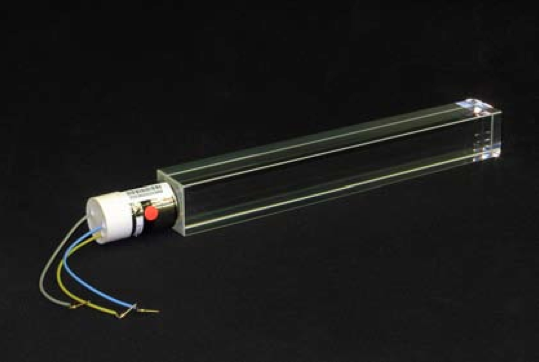
\includegraphics[height = 4cm]{lhc_cms/cms_ecal_crystal.png}
                    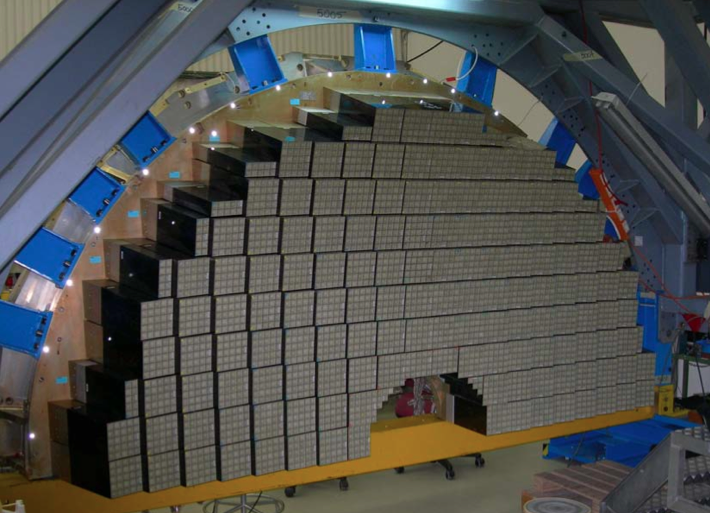
\includegraphics[height = 4cm]{lhc_cms/cms_ecal_endcap.png}
                    \caption{Picture of a PbWO$ _4 $ crystal (left) used in the ECAL with its photomultiplier, and of the endcap ECAL (right) showing the crates in which the crystals are placed \Cite{CMS_at_LHC}.}
                    \label{fig:lhc_and_cms__cms_ecal_view}
                \end{figure}

                In CMS, the ECAL is composed of PbWO$ _4 $ crystals, acting both as interaction media and as scintillators, attached to photomultipliers to amplify the relatively small amount of photons they emit. The crystals measure 2.2 cm x 2.2 cm, which is equivalent to one Molière radius $ R_M $, by 23 cm, which corresponds to several radiation lengths $ X_0 $. Figure \ref{fig:lhc_and_cms__cms_ecal_view} shows one of these crystals (left), the crates that hold them, and their disposition in the endcap (right). The number of photons collected is proportional to the energy deposited in the calorimeter modulo a correction factor due to the aging of the material. The ambient radiation causes the crystals to become opaque and release less photons which in turn implies a constant need for recalibration of the detectors.

            \subsubsection{Hadronic Calorimeter}

                Where the ECAL relies on radiative processes to detect particles, the HCAL uses strong interactions between the hadrons and the material to create hadronic cascades. These are much longer than electromagnetic showers, requiring longer detectors. The most created particles are pions as they are the lightest hadrons. This induces an electromagnetic component as the $ \pi^0 $ principal decay channel is $ \pi^0 \rightarrow \gamma \gamma $. This creates a problem, as the response of the material can be different for the hadronic and electromagnetic component. \\

                Figures \ref{fig:lhc_and_cms__cms_hcal_view} are a picture of a section of the barrel HCAL representing the absorber (golden plates) with the scintillator in between and of the installation of the barrel HCAL in CMS. The HCAL is composed of an alternation of 16 layers of absorbers, made out of 40 to 70 mm thick steel plates and 50 to 56 mm thick 70\% Cu and 30\% Zn alloy plates, and 3.7 to 9 mm thick plastic scintillators. When particles hit the detectors perpendicularly, they have to travel through 79 cm of matter equivalent to 5.82 interaction lengths $ \lambda_I $. The barrel HCAL is divided into 72 segments in $ \phi $ and 16 $ \eta $ sectors while the endcap HCAL has 36 and 72 $ \phi $ segments for the inners and outers rings respectively, and 14 $ \eta $ sectors.

                \begin{figure}[h!]
                    \centering
                    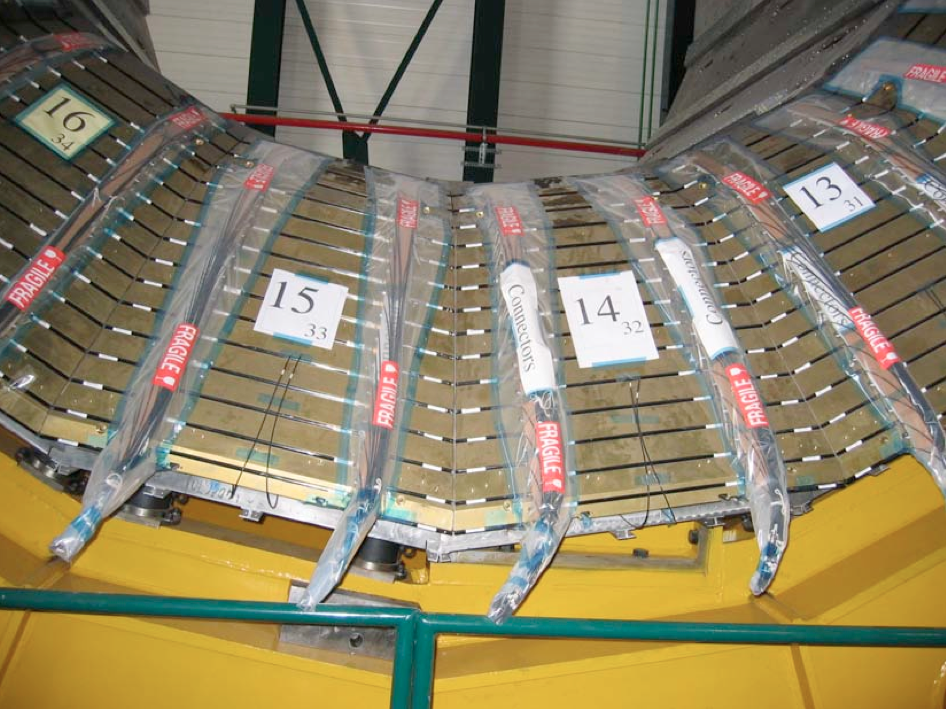
\includegraphics[height = 5cm]{lhc_cms/cms_hcal.png}
                    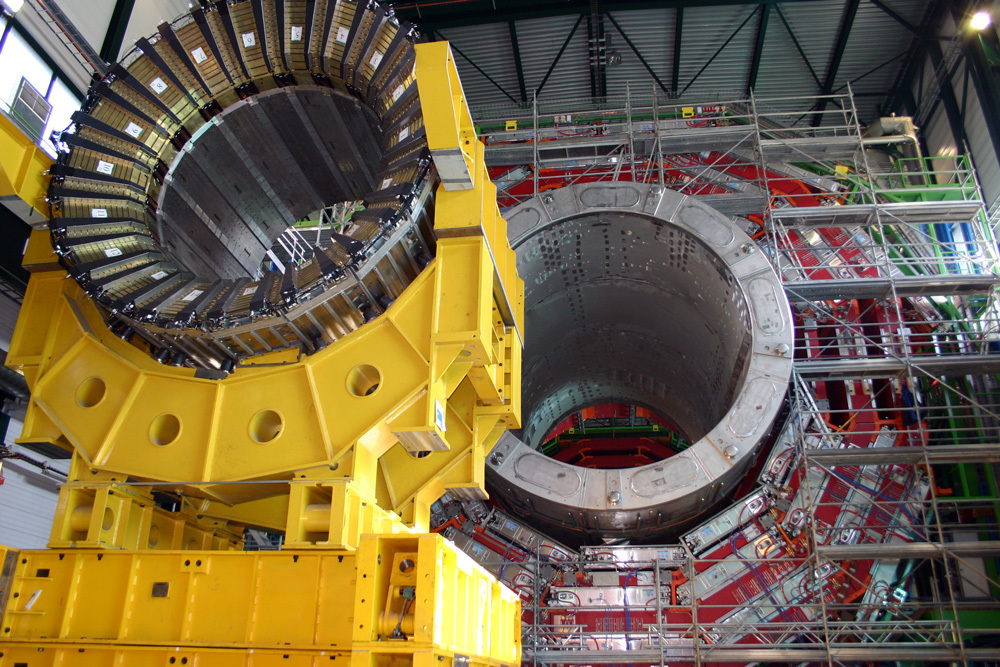
\includegraphics[height = 5cm]{lhc_cms/cms_hcal_install.jpg}
                    \caption{Picture of the barrel HCAL composed of several dense absorber (golden plates) and smaller scintillators placed in between (left) \Cite{CMS_at_LHC}, and installation in CMS of the barrel HCAL (right) \Cite{CMS_HCAL_Install}}
                    \label{fig:lhc_and_cms__cms_hcal_view}
                \end{figure}    

            \subsubsection{System Performances}  
            \label{sec:lhc_and_cms__calorimeters_system_performances}   

                The CMS ECAL's energy resolution is \Cite{CMS_Performances}
                \begin{equation}
                    \left( \frac{\sigma_E}{E} \right)^2 = \left( \frac{2.8\%}{\sqrt{E}} \right)^2 + \left( 0.30\% \right)^2 + \left( \frac{0.12}{E} \right)^2 \ ,
                \end{equation}      
                where $ E $ is given in GeV. The CMS HCAL's energy resolution is
                \begin{equation}
                    \left( \frac{\sigma_E}{E} \right)^2 = \left( \frac{120\%}{\sqrt{E}} \right)^2 + \left( 6.9\% \right)^2 \ .
                \end{equation}      

        \subsection{Superconducting Magnet}

            The intense magnetic field of CMS is created by cooling a solenoid down to 4.5 K, temperature at which the metal becomes supra-conductive, and by passing strong currents through it. The resulting field is uniform inside the solenoid but more complex outside, as shown in Figure \ref{fig:lhc_and_cms__cms_magnetic_field} which represents the measured magnetic field. The constant and strong field in which the tracker is placed allows it to measure the particles' transverse momentum with high-precision (resolution of less than 1\% in the tracker as seen in Figure \ref{fig:lhc_and_cms__cms_tracker_performances}). The intensity of the field is of 3.8 T inside the solenoid and typically 2 T outside the solenoid. \\

            \begin{figure}[h!]
                \centering
                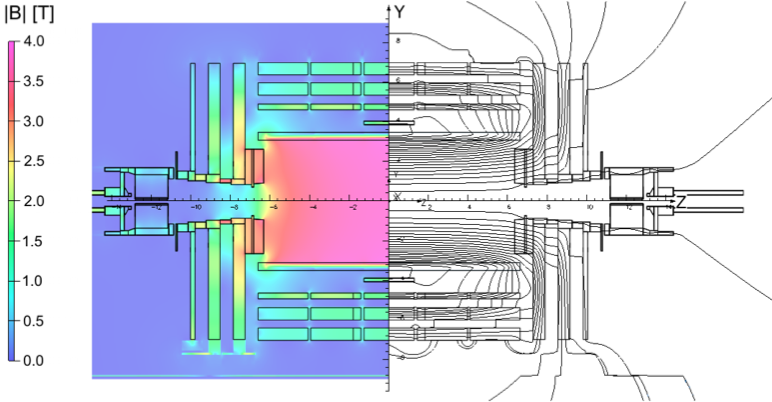
\includegraphics[width = 12cm]{lhc_cms/cms_magnetic_field.png}
                \caption{Field map of the magnetic field of CMS measured using cosmic rays \Cite{CMS_B_Field}.}
                \label{fig:lhc_and_cms__cms_magnetic_field}
            \end{figure} 

            Having the calorimeters inside the magnet improves the energy resolution as particles have less matter to travel through before reaching them, but increases the size of the solenoid. Due to the technical difficulty to build large magnets, the muon chambers are placed on the outside. This layout has the advantage to use the magnet as barrier for most particles escaping the calorimeters, ensuring that only muons will be detected by the muon system.

        \subsection{Muon Spectrometer}

            Currently, the CMS muon system \Cite{CMS_at_LHC, CMS_Performances} is composed of three different types of gaseous detectors: \emph{Drift Tube} (DT), \emph{Cathode Strip Chamber} (CSC), and \emph{Resistive Plate Chamber} (RPC).

            Like all the CMS detectors, the muon system is divided into two regions: the barrel ($ | \eta | $ < 1) and the endcaps (1 < $ | \eta | $ < 2.4). The chambers are regrouped into stations attached to the wheels of CMS. The barrel stations contain DTs (identified by MBn) and RPCs while the endcaps stations hold CSCs (identified by MEx/y) and RPCs (identified by REn), as represented in Figure \ref{fig:muon_chambers__placement}. For financial reasons, the RPCs were not installed for the LHC's start-up in the 1.6 < $ | \eta | $ < 2.4 region where only CSCs are present. 

            \begin{figure}[h!]
                \centering
                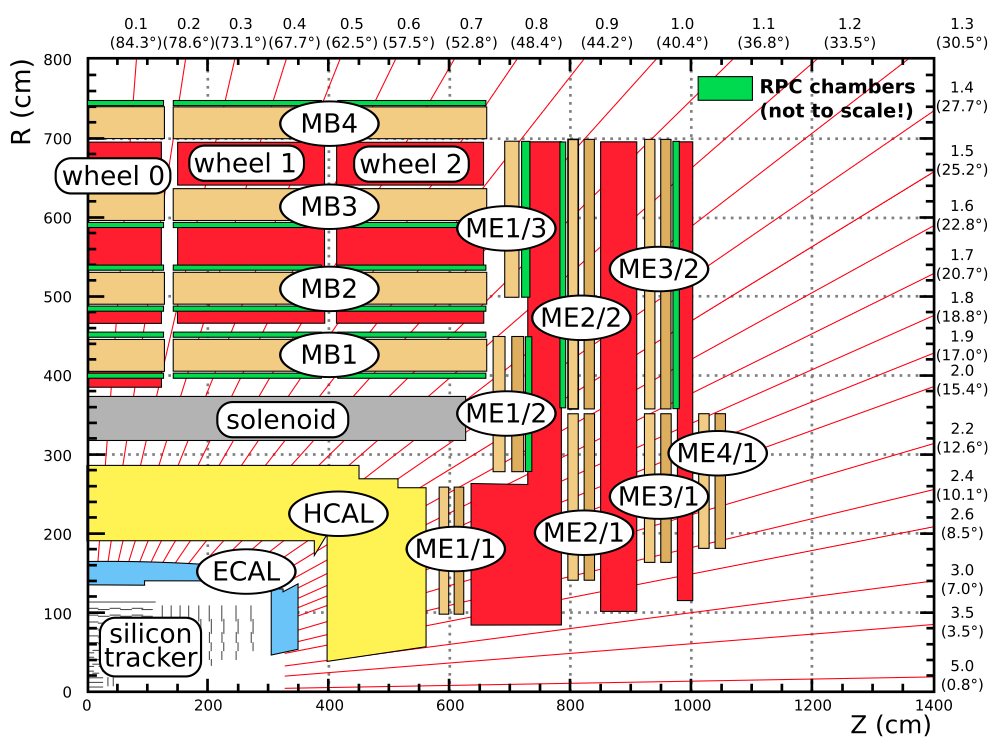
\includegraphics[width = 13cm]{lhc_cms/cms_chambers_placement.png}
                \caption{Disposition of the muon chambers inside CMS. MBn refer to DTs, MEn to CSCs and the green lines to RPCs \Cite{CMS_Upgrades}.}
                \label{fig:muon_chambers__placement}
            \end{figure}    

            The barrel is composed of 5 wheels on which 4 layers of detectors are attached, each divided into 12 stations along $ \phi $. The endcaps have 4 layers of detectors divided into 1, 2 or 3 rings partitioned into 36 or 72 stations that overlap to ensure maximum efficiency. Figure \ref{fig:muon_chambers__cms_endcap} shows the first station of the muon endcap, ME1. The inner ring, called ME1/1 is hidden by the so-called \emph{nose}, in black. The two outer rings, ME1/2 and ME1/3 are well visible. In ME1/2, we can observe the overlap between the chambers. \\

            \begin{figure}[p!]
                \centering
                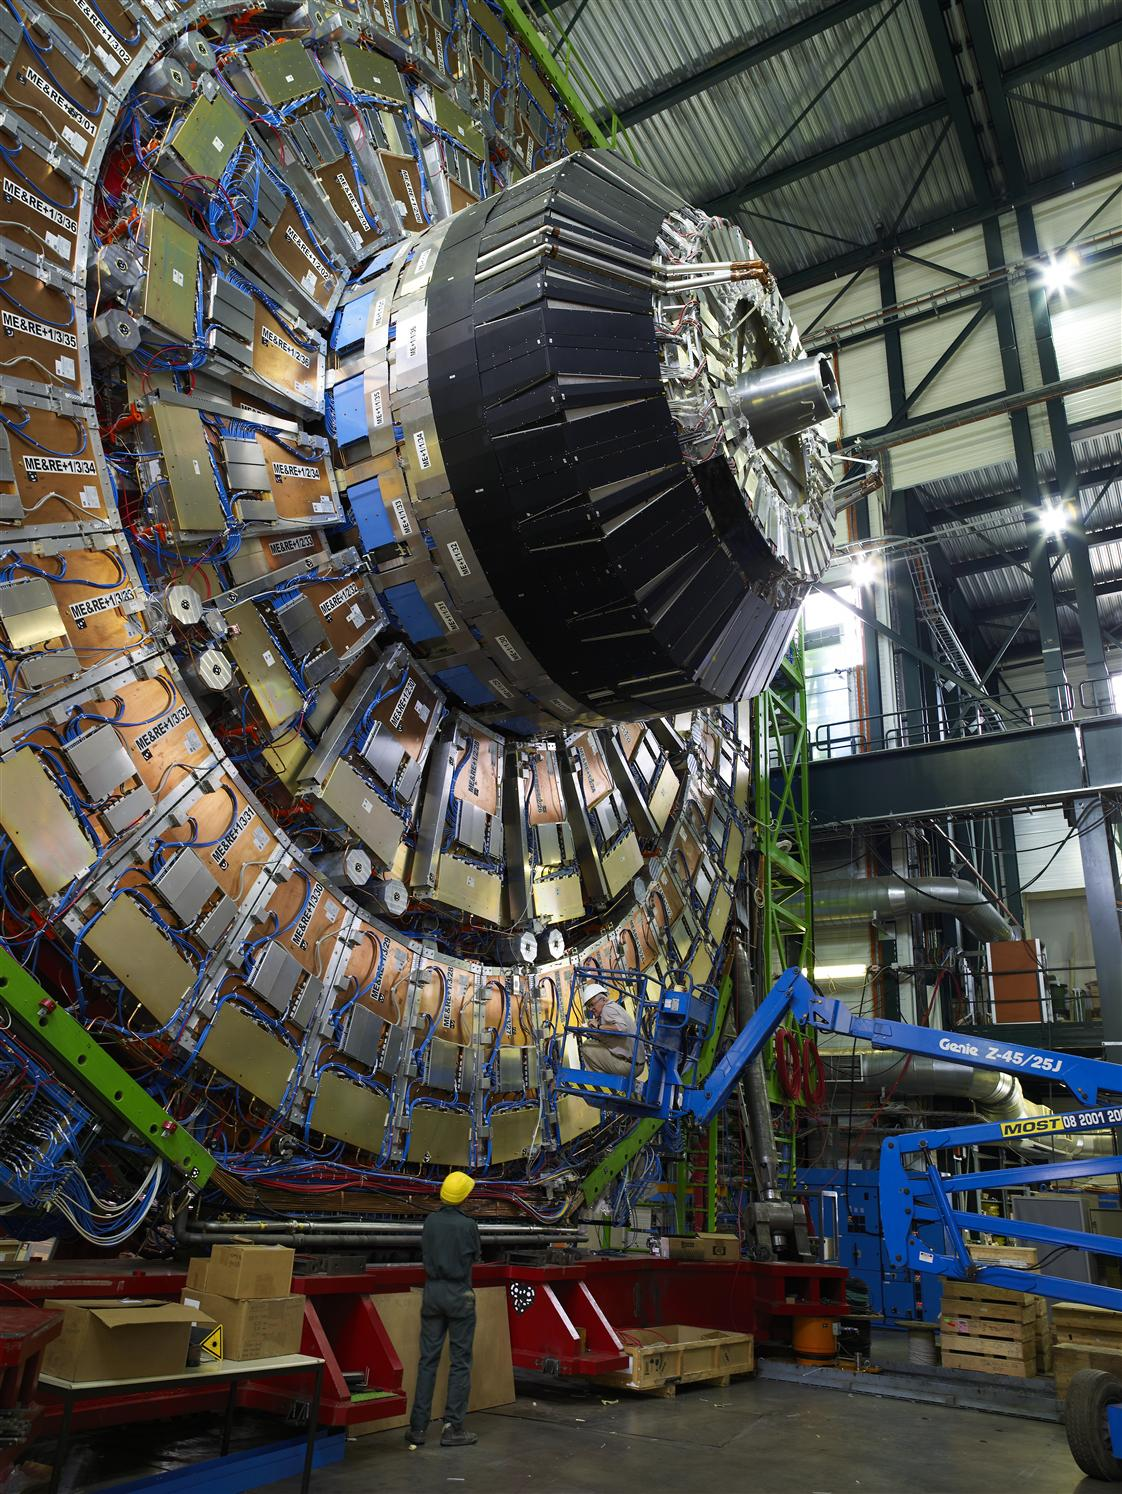
\includegraphics[width = 16.5cm]{lhc_cms/cms_endcap_view.jpg}
                \caption{Picture of one of the endcaps' yokes. We can observe the two outer rings, ME1/2 and ME1/3. Chambers of the inner ring, ME1/1, are hidden inside the \emph{nose}, in black \Cite{Fig_CMS_Endcap}.}
                \label{fig:muon_chambers__cms_endcap}
            \end{figure}    

            The use of two different kinds of detectors in each station ensures that the system meets the required detection efficiency for muons imposed by CMS. This redundancy is crucial to select and reconstruct events with high momentum muons in the final state, signature of the Brout-Englert-Higgs boson's decay and of many processes of new physics, including super-symmetry.

            \subsubsection{Drift Tubes}

                DTs are rectangular parallelepiped detectors composed of an anode wire stretched between two cathode strips as represented in Figure \ref{fig:muon_chambers__dt}. The chambers are 2.4 m long by 13 mm height by 42 mm wide. A strong electric field (of the order of 1.5 kV cm$ ^{-1} $) is formed by applying a high voltage difference between the electrodes, causing the electrons and ions to drift into the gas, and provoking avalanches near the anode. The two electrodes placed near the anode help flatten the electric field and improve the charges' drift. \\

                \begin{figure}[h!]
                    \centering
                    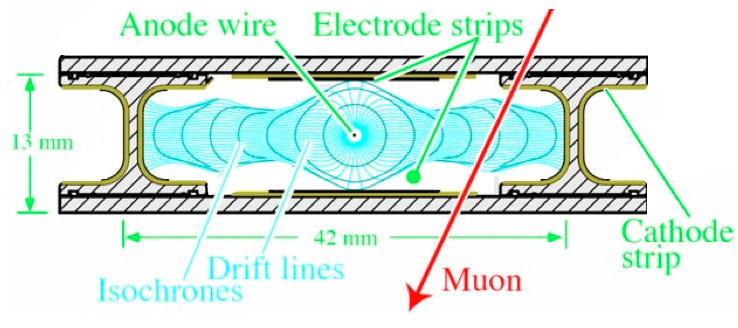
\includegraphics[width = 8cm]{lhc_cms/cms_dt.png}
                    \caption{Schematic view of a drift cell along with the electric field line \Cite{CMS_at_LHC}.}
                    \label{fig:muon_chambers__dt}
                \end{figure}

                Four DTs are assembled to create a \emph{Super Layer} (SL), and two or three SLs compose a DT module. Each SL has a spatial resolution of 100 \um{} in the direction perpendicular to the wire. To improve global precision, two SLs are used to measure the $ \phi $ coordinate and sometimes one additional SL is used to measure $ \eta $. DT modules have a time resolution of 3 ns. Their rather large size limits their rate capabilities, explaining why they are only present in the barrel where particles' fluxes are lower (< 10 Hz cm$ ^{-2} $).

            \subsubsection{Cathode Strip Chambers}

                CSCs are trapezoidal multiwire proportional chambers placed in the endcaps of CMS. Multiple anode wires (about 1000 spaced by 3.2 mm) are stretched radially in the chamber above perpendicularly placed cathode strips (typically 80 separated by a pitch of 8.4 mm on the narrow side and 16 mm on the large side) as depicted in Figure \ref{fig:muon_chambers__csc}. As for the DTs, an electric field is formed between the wires and the strips, accelerating the electrons and forming the avalanches near the anodes. By reading-out both electrodes, the CSCs provide a measurement of both coordinates.

                \begin{figure}[h!]
                    \centering
                    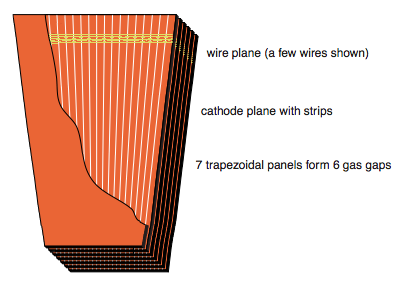
\includegraphics[height = 4.5cm]{lhc_cms/cms_csc.png}
                    \caption{A representation of a CSC with its wires and strips \Cite{CMS_Performances}}
                    \label{fig:muon_chambers__csc}
                \end{figure}

                One CSC module is made out of six chambers put together (7 cathode planes and 6 wire planes). Due to the large number of readout channels in these modules, the spatial resolution is as good as 33 \um{} for ME1/1 and ME1/2, and 80 \um{} for the other stations. The time resolution for one cathode plane is 11 ns that can be brought down to the order of 5 ns when combining the measurements of all the planes. The largest CSC modules, ME2/2 and ME3/2, are 3.4 m by 1.5 m. \\ 

                Note that the two dimensional readout configuration can create ambiguities called \emph{ghosts particles} as shown in Figure \ref{fig:muon_chambers__ghosts}. When two particles hit the chamber (left), four possibilities arise when reading the output signal (right). Two of them correspond to real particles, and the two others to ghost particles. It is easy to see that for $ n $ particles interacting in the chamber, $ n^2 $ particles can be reconstructed. This limits the rates at which the CSCs can function to 1 kHz cm$ ^{-2} $. 

                \begin{figure}[h!]
                    \centering
                    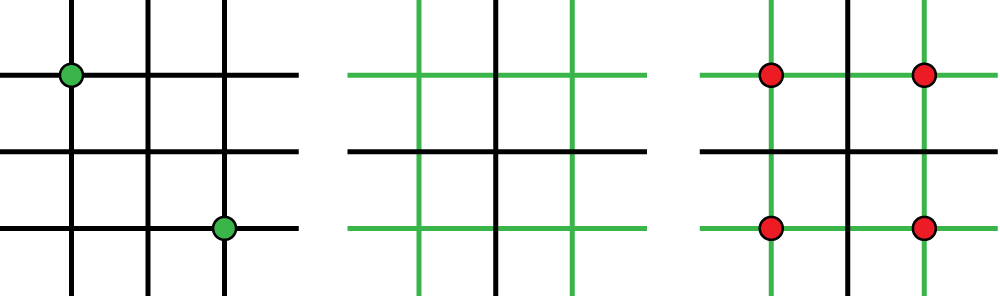
\includegraphics[width = 8cm]{lhc_cms/cms_csc_ghost.png}
                    \caption{Ambiguities arise when more than one particle hit the chamber at the same time.}
                    \label{fig:muon_chambers__ghosts}
                \end{figure}
        
            \subsubsection{Resistive Plate Chambers}

                RPCs, represented in Figure \ref{fig:muon_chambers__rpc}, are gaseous parallel plate detectors. They consist of two parallel plates, made out of bakelite with a high resistivity (10$ ^{10} $ to 10$ ^{11} $ $ \Omega $ cm) separated by a gas gap of a few millimeters. The outer surfaces of the resistive materials are coated with conductive graphite to form the HV and ground electrodes. Due to the fact that ions and electrons never come in contact with the electrodes, the evacuation time can be of importance if too many charges are produced. Therefore, the gain of the detectors are reduced and most of the amplification is done by the readout electronics and not by avalanches. This allows the RPCs to run at rates up to 1 kHz cm$ ^{-2} $, while maintaining an excellent time resolution down to 1 ns. On the other hand, they have a poor spatial resolution of the order of 1 mm. \\

                \begin{figure}[h!]
                    \centering
                    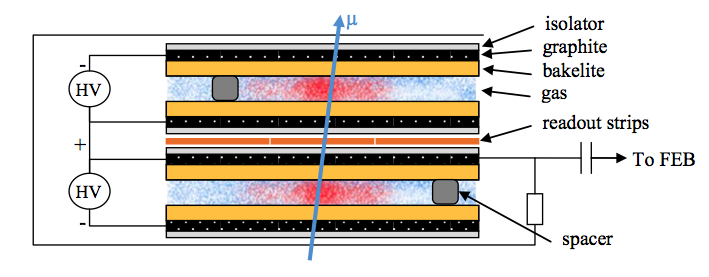
\includegraphics[width = 10cm]{lhc_cms/cms_rpc.png}
                    \caption{Representation of an RPC with two gas gaps for one readout strip plane \Cite{These_Karol}.}
                    \label{fig:muon_chambers__rpc}
                \end{figure}

                Since the RPCs can operate at high hit rate, they are used in both the barrel and the endcaps as trigger system. In the barrel, RPCs are rectangular chambers covering the DTs, while in the endcaps, they have a trapezoidal shape like the CSCs.

            \subsubsection{System Performances}
            \label{sec:muon_chambers__system_performances}

                Figure \ref{fig:muon_chambers__performances} represents the resolution on the transverse momentum $ p_T $ of muons as a function of the pseudo-rapidity $ \eta $ for the muon system in standalone (left) and combined with the tracker's data (right). The standalone system suffers from discontinuities in $ \eta $ when transitioning from the barrel to the endcaps ($ | \eta | $ = 1) or between stations in the endcaps where particles are not detected. These imprecisions can be removed by considering data from the trackers, which also improves the overall precision by a factor of 10. For a muon with a transverse momentum of 10 \GeVc{}, the resolution goes down from about 10\% in the standalone reconstruction to about 1\% when considering the tracker.

                \begin{figure}[h!]
                    \centering
                    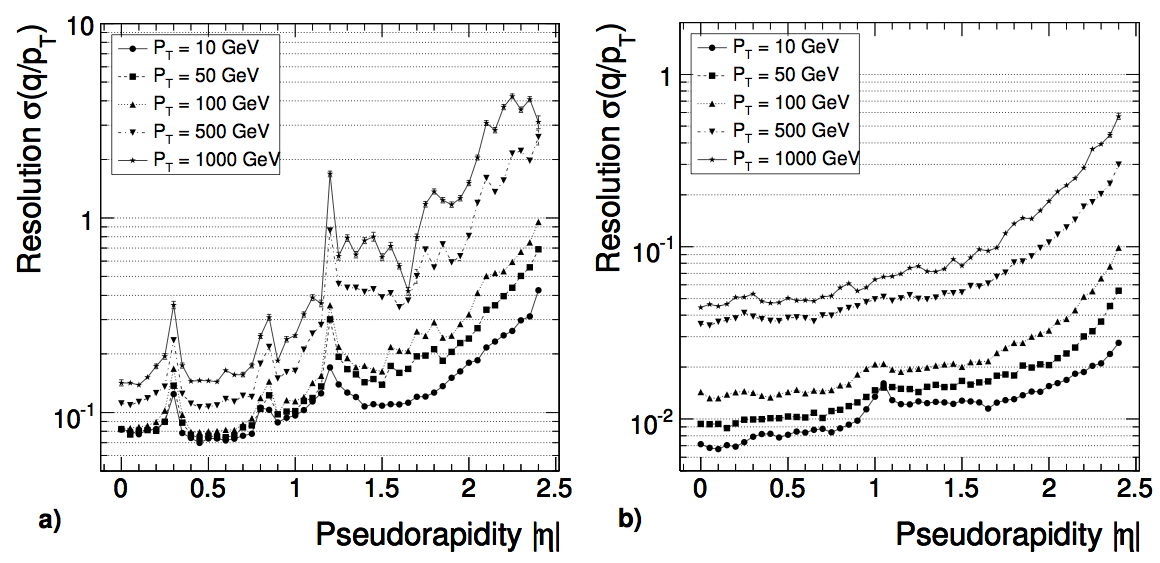
\includegraphics[width = 13cm]{lhc_cms/cms_muon_performances.png}
                    \caption{Resolution on the transverse momentum $ p_T $ of muons as a function of the pseudo-rapidity $ \eta $ for the muon system in standalone (left) and combined with the tracker's data (right) \Cite{CMS_Performances}.}
                    \label{fig:muon_chambers__performances}
                \end{figure}            

        \subsection{Trigger System}

            With the LHC running at a rate of 40,000,000 collisions per second, the amount of data produced by CMS is considerable ($ \sim $ 40 TB s$ ^{-1} $). We do not yet have the technology to transfer nor handle all this information. Therefore, a selection of interesting events has to be done in order to reduce the transfer's rate. The decision to keep or drop an event is taken by the CMS trigger system which includes two stages: the \emph{Level-1 Trigger} (L1 Trigger) and the \emph{High Level Trigger} (HLT) \Cite{CMS_at_LHC}. \\

            Figure \ref{fig:trigger_system_and_reconstruction_algorithms__rates} depicts the different stages of the trigger and the maximal rate of events kept by each one of them, starting at 40 MHz and ending at 100 Hz. The kept events are sent and stored in multiple locations around the world (called \emph{Tiers}) where physicists can analyze them.

            \begin{figure}[h!]
                \centering
                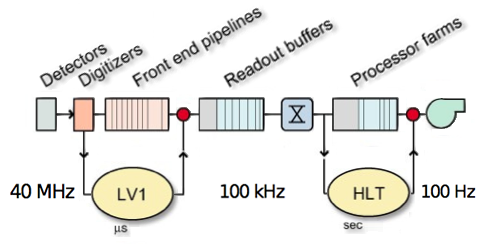
\includegraphics[width = 10cm]{lhc_cms/trigger_rates.png}
                \caption{Data rates at each stage between the detectors and the data storage center. \Cite{CMS_Trigger_System}}
                \label{fig:trigger_system_and_reconstruction_algorithms__rates}
            \end{figure}    

            \subsubsection{Level-1 Trigger}

                The L1 Trigger is the first stage of selection of CMS and has to be able to handle all events successively. Therefore, it has to take a "keep or drop" decision every 25 ns (time between two BXs). The system is composed of dedicated electronic chips for each detector placed either on CMS or in the service caverns next to it, to protect them from radiations. A diagram of the L1 Trigger's decision flow is shown in Figure \ref{fig:trigger_system_and_reconstruction_algorithms__l1}. The decision is first taken locally by small groups of muon chambers and calorimeters before being sent to the \emph{Global Muon Trigger} (GMT) \Cite{Trigger_Muon} and \emph{Global Calorimeter Trigger} (GCT) respectively, that analyze the event over all the regions. Finally, the GMT and GCT send their keep/drop signal to the \emph{Global Trigger} (GT). As represented, the tracker is not involved in this first stage selection due to the time needed to reconstruct and transfer the output data. \\

                \begin{figure}[h!]
                    \centering
                    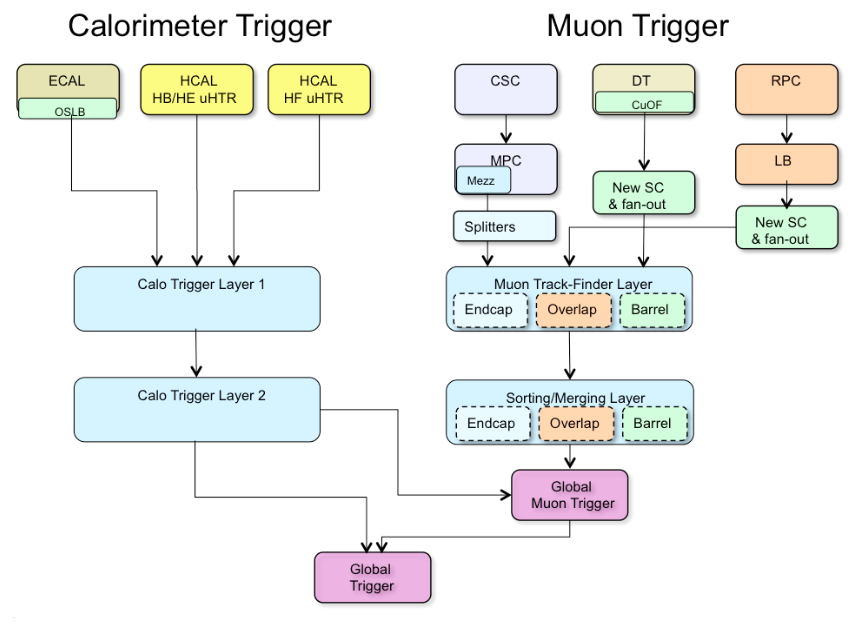
\includegraphics[width = 10cm]{lhc_cms/l1.png}
                    \caption{L1 Trigger decision flow of CMS before data is being transfered to the DAQ \Cite{CMS_at_LHC}.}
                    \label{fig:trigger_system_and_reconstruction_algorithms__l1}
                \end{figure}

                When a collision occurs, every 25 ns, the system reads out the response of every detector and stores it in a buffer that holds the last 128 events. Consequently, the algorithms have a maximum of 3.2 \us{} to process each event and return their decision. This also allows the decision taking process to be differed between the different triggers (GMT and GCT) as the particles take a certain time to travel from the IP to the various detectors. Once an algorithm has made a decision, it sends a one bit signal to the GMT or GCT. When all the detectors have responded, the GT either drops the event or tells the DAQ system to transfer it to the HLT. \\

                As the L1 Trigger only relies on the calorimeters and on the muon system, the events' selection is done according to the signature and transverse energy left in the calorimeters, and to the transverse momentum reconstructed by the muon system. Only the transverse components of the energy and the momentum are considered as they reflect the physics of the event. Indeed, when the protons collide, the fraction of energy put at play in the interaction is not the same. Therefore, the produced particles will be boosted along \axis{Z} according to these differences, while the total transverse momentum should remain null as the collisions are head to head.

            \subsubsection{High Level Trigger}

                The HLT is composed of a farm of computers running reconstruction software that can perform complex calculations. Due to the filtering made by the L1 Trigger, the incoming data rate is lower (100 kHz), allowing for a longer processing time, of the order of 1 s. If an event passes through the multiple filters and is accepted, it is send to the storage unit and made available for analysis. Since this work aims to study track reconstruction performed at L1, the HLT will not be further reviewed.

            \subsubsection{Muon System Trigger}

                The different muon chambers have their own trigger system which benefits from the detectors strengths. DTs and CSCs have excellent spatial resolution (respectively of the order of 100 and 80 \um{}) and will therefore be used to filter the events according to their transverse momentum. RPCs on the other hand have great timing capabilities (down to 1 ns) which yields good BX assignment. By combining the DTs and RPCs in the barrel, and the CSCs and RPCs in the endcaps, the GMT can reconstruct event with a multitude of muons in the final state.

                \paragraph{Local Muon Trigger}

                    DT modules are divided into smaller segments as represented on the left in Figure \ref{fig:trigger_system_and_reconstruction_algorithms__dt_local}. Each couple of layers (AB, AC, AD, etc) is used to compute the position $ \mathbf{x} $ and the angle $ \phi_b $ of the track by measuring the arrival time of the signals to the anode. The further away a particle passes from the wire, the longer the drift time is, hence the time at which the signals are detected. If the values match for several couples, the segment is considered to represent a valid track and marked as such. The number of couples that return the same value defines the quality of the track. If an ambiguity appears, the parameters with the best quality are selected. \\       

                    \begin{figure}[h!]
                        \centering
                        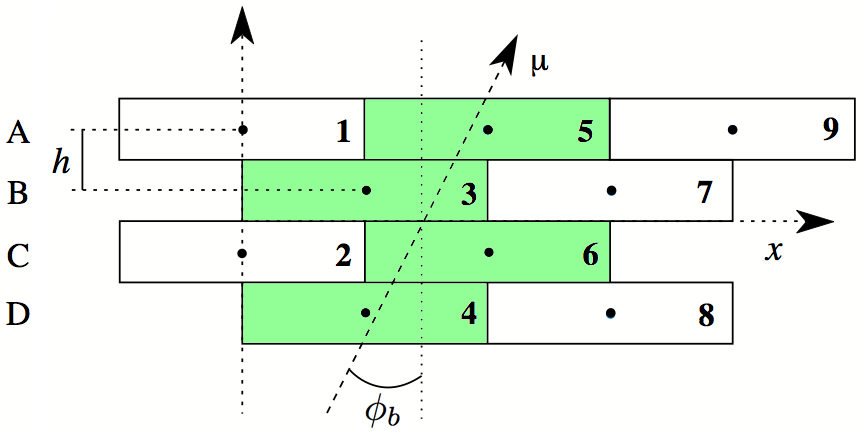
\includegraphics[height = 3.5cm]{lhc_cms/l1_dt_local.png}
                        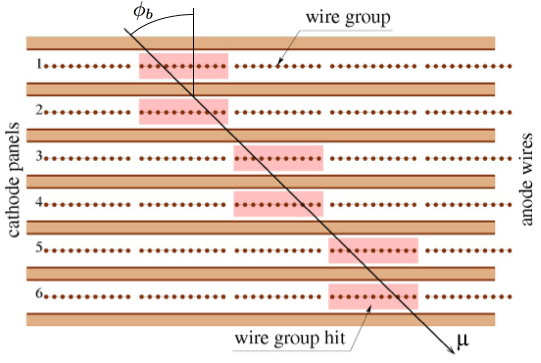
\includegraphics[height = 3.5cm]{lhc_cms/l1_csc_local.png}
                        \caption{DTs' local trigger measuring the particle's incident angle using the ions' drift time (left) \Cite{CMS_at_LHC}; CSCs' local trigger relying on the multiple layers to measure the particle's incident angle (right) \Cite{Trigger_Muon}.}
                        \label{fig:trigger_system_and_reconstruction_algorithms__dt_local}
                    \end{figure}

                    The same is done in CSC modules using the six planes of anode wires and seven planes of cathode strips, as seen on the right in Figure \ref{fig:trigger_system_and_reconstruction_algorithms__dt_local}. Due to the short amount of time available to run the reconstruction, anode wires are grouped by 5 to 16 by performing a logical \emph{OR} of the binary readout result.

                \paragraph{Global Muon Trigger}

                    Once tracks have been reconstructed locally, the TF matches the different stations by comparing their hits. Figure \ref{fig:trigger_system_and_reconstruction_algorithms__dt_global} shows the pairwise matching between stations (left), the muon track (left; green), and the reconstructed track in the transverse plane (left; red). First, using the local reconstructed angle $ \phi_b $ of the track (middle), the parameters are extrapolated between layers (right) by using predefined parameters stored in LUTs for all the possible matching segments
                    \begin{equation}
                        \phi_{extrapolation} = \phi_b + \phi_{deviation} \ ,
                    \end{equation}
                    where $ \phi_{extrapolation} $ is the extrapolated parameter, and $ \phi_{deviation} $ is the deviation in $ \phi $ between two detection planes. If the extrapolation is close to the measurement, within a predefined range (right; blue), the site is added to the track and the propagation continues towards the next station. This method can result in more than one reconstructed track, which is why only the four tracks with the highest quality (best match between extrapolation and measurements, most matches, etc) are kept. Finally, an estimation of the transverse momentum in function of the bending angle is done.
                    
                    \begin{figure}[h!]
                        \centering
                        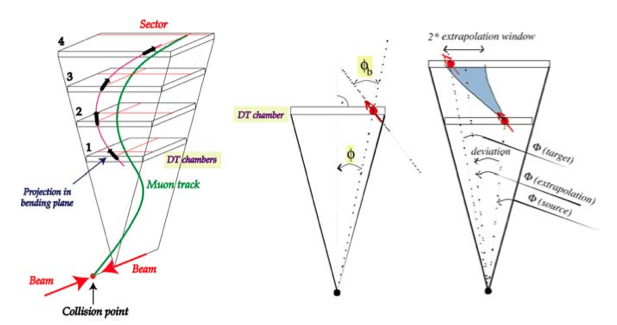
\includegraphics[width = 12cm]{lhc_cms/l1_track_finder.png}
                        \caption{Reconstructed trajectory by the Track-Finder using pairwise matching between the stations \Cite{CMS_at_LHC}.}
                        \label{fig:trigger_system_and_reconstruction_algorithms__dt_global}
                    \end{figure}

        \subsection{Data Acquisition System}

            Explain principles of DAQ

            \subsubsection{Detectors Readout}

                DAQ readout structure (front-end, back-end in cavern, ...)

            \subsubsection{Event Builder}

                Event reconstruction from multiple sub-detectors

            \subsubsection{Event Filter}

                Event filtering (HLT) and storage

            \subsubsection{Run, Control, and Monitoring Infrastructure}

                System control (RCMS, XDAQ, ...)


	\cleardoublepage

	\chapter{The CMS Upgrades}
\label{chap:upgrades}

    Present the upgrades

    \section{Future Plans}

        Explain why upgrades are required

    \section{The CMS GEM Project}

        Short intro to the GEM project

        \subsection{Physics Motivations}

            Why we need an upgrade and why the GEMs are good

        \subsection{Triple-GEM Detector Design}

            How GEMs function

            \subsubsection{Gas Electron Multiplier Principles}

                About a Single GEM and how they work

            \subsubsection{GEM Foils Production}

                About how GEMs are produced

            \subsubsection{Chambers Mechanical Design}

                About how the GEMs are assemble

        \subsection{Detector Performance}

            How GEMs perform

            \subsubsection{Detection Efficiency}

                Detection Duh

            \subsubsection{Spatial Resolution}

                Spatial Duh

            \subsubsection{Time Resolution}

                Time Duh

            \subsubsection{Particle Rate Capability}

                Rate Duuh

        \subsection{Detector Testing and Installation}

            What has been tested in the past and will be done

            \subsubsection{Test Beam Campaigns}

                About previous test beam campaigns

            \subsubsection{Slice Test Integration}

                About the slice test

            \subsubsection{Phase2 Installation}

                About Phase2

            \subsubsection{Phase2 Installation}

                About Phase3

        \subsection{Status of the GEM Project}

            Current status of the GEM project

    \section{The Phase2 Outer Tracker Upgrades}

        About the Phase2 Outer Tracker Upgrades

        \subsection{Physics Motivations}

            About why we want this

        \subsection{New Tracker Geometry}

            How the modules are arranged in the detector

        \subsection{pT Modules}

            Describe what we call pT Modules

            \subsubsection{Pixel and Strip Sensors}

                Describe the sensors

            \subsubsection{PS and 2S Modules}

                Describe the PS and 2S Modules

            \subsubsection{Readout Chip}

                About the CBC, GBT, ...

        \subsection{Data Reduction and Formatting}

            How the data is formatted

            \subsubsection{Trigger Stubs}

                For the trigger

            \subsubsection{Tracking Clusters}

                For the tracking

        \subsection{Level-1 Track Trigger}

            About the Track Trigger

	\cleardoublepage

	\chapter{The GEM Data Acquisition System for the Test Beam}
\label{chap:gem_daq_test_beam}

    About the V1

    \section{Objectives of the Test Beam}

        What we wanted to achieve

    \section{System Components}

        About the components

        \subsection{VFAT2 Front-End Chip}

            Describe VFAT2

        \subsection{GEB Routing Board}

            Describe GEB

        \subsection{OptoHybrid Concentrator}

            Describe VFAT2

        \subsection{uTCA Standard}

            Describe uTCA Technology

        \subsection{GLIB Back-End Mezzanine}

            Describe GLIB

    \section{System Architecture}

        Describe system used for the test beam, how the components fit together

    \section{Firmware and Software Development}

        Present the firmware

        \subsection{Front-end Control}

            Present the control of the VFAT2 through I2C

        \subsection{Front-end Data Readout}

            Present the readout of the tracking data

        \subsection{Trigger and Clocking Scheme}

            Present the timing and trigger scheme

        \subsection{Front-end / Back-end Communication}

            Optical communication

        \subsection{Run and Control Communication}

            IPBus protocol

        \subsection{Data Tacking Process}

            Data readout from the GLIB

    \section{Test Beam Campaign}

        Short intro on Test Beam

        \subsection{Test Beam Setup}

            Present the setup at the test beam

        \subsection{Trigger Signal and Synchronisation}

            How the system is trigger and synchronized

        \subsection{System Monitoring}

            The python scripts

        \subsection{Analysis of the Results}

            Present the data results

            \subsubsection{Threshold Scan}

                Threshold Scan

            \subsubsection{Latency Scan}

                Latency Scan

            \subsubsection{Tracking Data and Beam Profile}

                Beam Profile

            \subsubsection{Cluster Size}

                Cluster size

    \section{Conclusion}

        Conclude on this design



	\cleardoublepage

	\chapter{The GEM Data Acquisition System for the Slice Test}
\label{chap:gem_daq_slice_test}

    About the V2

    \section{Requirements for the Slice Test}

        What we need to add for the slice test

        \subsection{Radiation Hardness}

            Talk about radiation hardness

            \subsubsection{GBT Optical Link Architecture}

                Describe GBT

            \subsubsection{Versatile Link}

                Describe Versatile

            \subsubsection{SEU Mitigation}

                Describe possible SEU mitigation techniques

        \subsection{Integration in the CMS DAQ}

            What we need to do to integrate in the CMS DAQ System

            \subsubsection{AMC13 DAQ Module}

                Describe AMC13

    \section{DAQ Architecture}

        Describe the system used for the slice test

        \subsection{Hardware System}

            Describe the hardware

        \subsection{Software System}

            Describe the hardware

    \section{Readout Data Rates}

        Present computations presented for Paul about the data rates

        \subsection{Data Reduction Algorithms}

            Present the algorithms used to reduce data

        \subsection{Trigger Data Rates}

            Data rates at the trigger level

        \subsection{Tracking Data Rates}

            Data rates at the tracking level

    \section{Conclusion}

        Conclude on this section



	\cleardoublepage

	\chapter{The GEM Trigger System}
\label{chap:gem_trigger}

    \section{GEM-CSC Trigger}
        \subsection{Link to the Trigger Mother Board}
        \subsection{GEM CSC Impulsion Discrimination}

    \section{GEM Standalone Trigger}
        \subsection{Track Geometry}
        \subsection{Track Finding}
        \subsection{Track Fitting}

    \section{Trigger performance}
        \subsection{Muon Track Finder}
        \subsection{Muon Track Fitter}

    \section{Hardware implementation}

    \section{Trigger Integration}

	\cleardoublepage

	\chapter{Phase2 Tracker Local Reconstruction}
\label{chap:phase2_tracker}

    \section{The Phase2 Outer Tracker Upgrades}

        About the Phase2 Outer Tracker Upgrades

        \subsection{Physics Motivations}

            About why we want this

        \subsection{New Tracker Geometry}

            How the modules are arranged in the detector

        \subsection{pT Modules}

            Describe what we call pT Modules

            \subsubsection{Pixel and Strip Sensors}

                Describe the sensors

            \subsubsection{PS and 2S Modules}

                Describe the PS and 2S Modules

            \subsubsection{Readout Chip}

                About the CBC, GBT, ...

        \subsection{Data Reduction and Formatting}

            How the data is formatted

            \subsubsection{Trigger Stubs}

                For the trigger

            \subsubsection{Tracking Clusters}

                For the tracking

        \subsection{Level-1 Track Trigger}

            About the Track Trigger

    \section{CMSSW Workflow}

    \section{Local Reconstruction Workflow}

    \section{Phase2 Clusterizer Algorithm}

    \section{Results}

	\cleardoublepage

	\chapter{A Web DAQ System For Real-Time Data Visualisation}
\label{chap:web_daq}

    \section{Real-Time Systems}
    \section{New Web Technologies}
    \section{Proposed DAQ Architecture}

	\cleardoublepage

	\listoffigures
	\cleardoublepage

	\listoftables
	\cleardoublepage

	% \input{11_Annexes/abbreviations}
	% \cleardoublepage

	\printbibliography
	\cleardoublepage

\appendix

	% \input{11_Annexes/unbias}
	% \cleardoublepage

\end{document}
